\chapter{Settimana 2}

\NewDay{Prima sessione}{29/09/2020}
\section{Introduzione}

%\LogMark{Costruzione ponte di Wheatstone}{9:33}
%\begin{enumerate}
%    \item introduzione breve all'ambiente di lavoro TINA: nozioni pratiche di base. Poi ponte di %Weadsthone Mettiamo 4 resistenze. Din default 1 kohm. Clicca sul bottone destro, properties: label %per nome
%    \item connessione resistenze con "Wire"(la penna)
%    \item inserisco e connetto il generatore "Batteria", definiamo una massa (Lu, ston facendo una %cartella con un po' di immagini, poi te le passo, se intanto fai anche te, tipo incolla senza %tagliare su paint è meglio)OK, lo sto facendo pure io
%    \item n.b. uno dei problemi di TINA è nei mancati colegasmenti, ERC in Analisis per warnings and %errors, cliccandoci componenti inerenti.
%    \item su view puoi vedere quello cghe puoi vedere
%    \item help: component help: mi spiega che cosa e come posso cambiare le cose nel resistore. 
%\end{enumerate}

\NewSection{Ponte di Wheatstone in TINA}

\LogMark{Costruzione ponte di Wheatstone}{9:33}
Utilizzando l'ambiente TINA abbiamo realizzato lo schema del ponte di Wheatstone: abbiamo inserito 4 resistenze, un generatore di tensione continua e un amperometro. Abbiamo collegato i vari componenti con lo strumento \textit{Wire}, preoccupandoci di definire una massa.

\Orario{9:44} Successivamente abbiamo inserito i valori giusti per le resistenze e il generatore di tensione: R1 = 1k, R2 = 2, R3 = 1, RX = 3k, V1 = 5V.

\begin{figure}[H]
\caption{}
    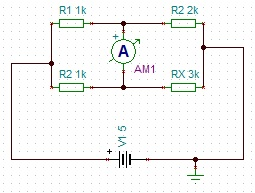
\includegraphics[width=5cm]{settimana_2/immagini/ponte_1.jpg}\label{fig::ponte}
    \centering
\end{figure}

\TODO{
    \sout{(Hw. 2) Inserisci i valori corretti e usa gli strumenti di analisi per verificare il valore di corrente sull'amperometro A.} Fatto il 03/10/20
}

\NewSection{Acquisiszione e realizzazione di diagramma di Bode}

\LogMark{Simulazione del filtro passa-basso}{16.15}
Il nostro scopo è simulare un circuito passa-basso RC con un software di simulazione e realizzazione di circuiti chiamato TINA. I componenti ed i collegamenti sono disposti come illustrato nella figura sottostante:
\begin{figure}[H]
\caption{}
    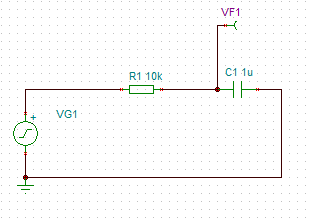
\includegraphics[width=5cm]{settimana_2/immagini/FiltroPassaBasso.png}
    \centering
\end{figure}
Utilizziamo il comando:
\begin{equation}
    Analysis \Rightarrow AC Analysis \Rightarrow AC Transfer Characteristic
\end{equation}
Si entra così all'interno di una finestra del tipo:
\begin{figure}[H]
\caption{}
    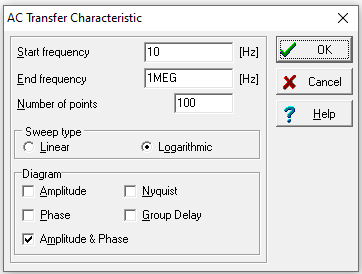
\includegraphics[width=5cm]{settimana_2/immagini/ACtransfer.png}
    \centering
\end{figure}
Mettiamo l'"end frequency" a 10 kHz e clicchiamo su "ok". Di seguito riportiamo i grafici risultanti, i quali riportano l'ampiezza e la differenza di fase fra segnale d'ingresso e d'uscita in funzione della frequenza del segnale sinusoidale in ingresso (questi grafici sono detti diagrammi di Bode):
\begin{figure}[H]
\caption{}
    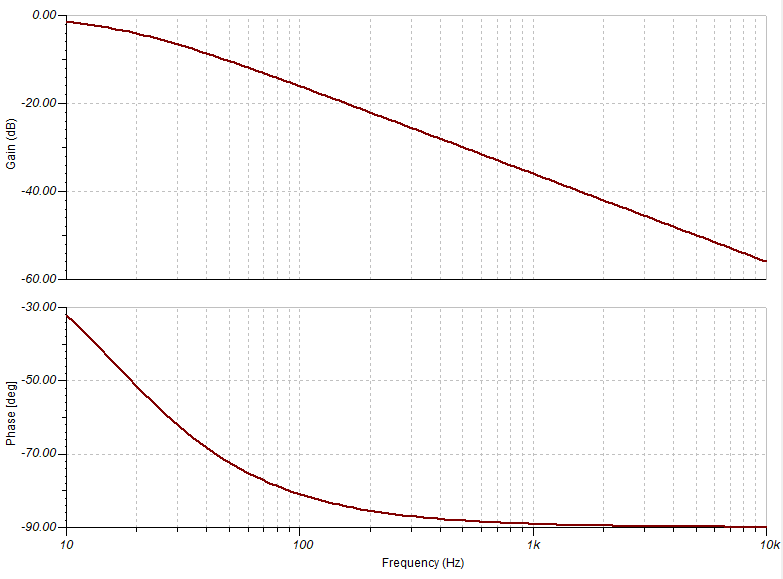
\includegraphics[width=5cm]{settimana_2/immagini/Bode.png}
    \centering
\end{figure}
Nella sezione che segue realizzeremo i diagrammi di Bode di segnali reali acquisiti da remoto.

\NewSection{Acquisizione dati corto circuito}
Alla pagina \textcolor{airforceblue}{\url{http://131.114.11.57:8000/BODE1.html}} abbiamo a disposizione il VI "bode\_*" che permette di generare ed acquisire segnali al fine di analizzare il comportamento di due circuiti: un corto-circuiro ed un filtro CRRC.

In particolare il VI si occupa di controllare un generatore di funzioni al fine di creare un segnale sinusoidale ed allo stesso tempo di acquisire i segnali $V_{in}$ e $V_{out}$ relativi ai circuiti in questione tramite la scheda DAQmx.

All'interno dell'interfaccia possiamo controllare i parametri di generazione e acquisizione, tra cui il range di frequenze che vogliamo spaziare.

Al termine della sequenza vengono visualizzati su un grafico i valori ricavati del guadagno e dello sfasamento di $V_{in}$ rispetto a  $V_{out}$, in funzione della frequenza.

\LogMark{acquisizione di prova}{17:08}
Per verificare il corretto funzionamento dell'apparato abbiamo eseguito un run preliminare sul corto circuito (\verb|ai0|), con i valori preimpostati ed un numero di misure impostato a 5 al fine di ottenere rapidamente dei risultati.

Come controllo visivo osserviamo che i guadagni sono concentratti attorno l'unità (come atteso), mentre gli sfasamenti risultano piccoli, ma risulta necessario prendere altri dati per trarre conclusioni circa il loro dandamento.

\begin{figure}[H]
\caption{}
    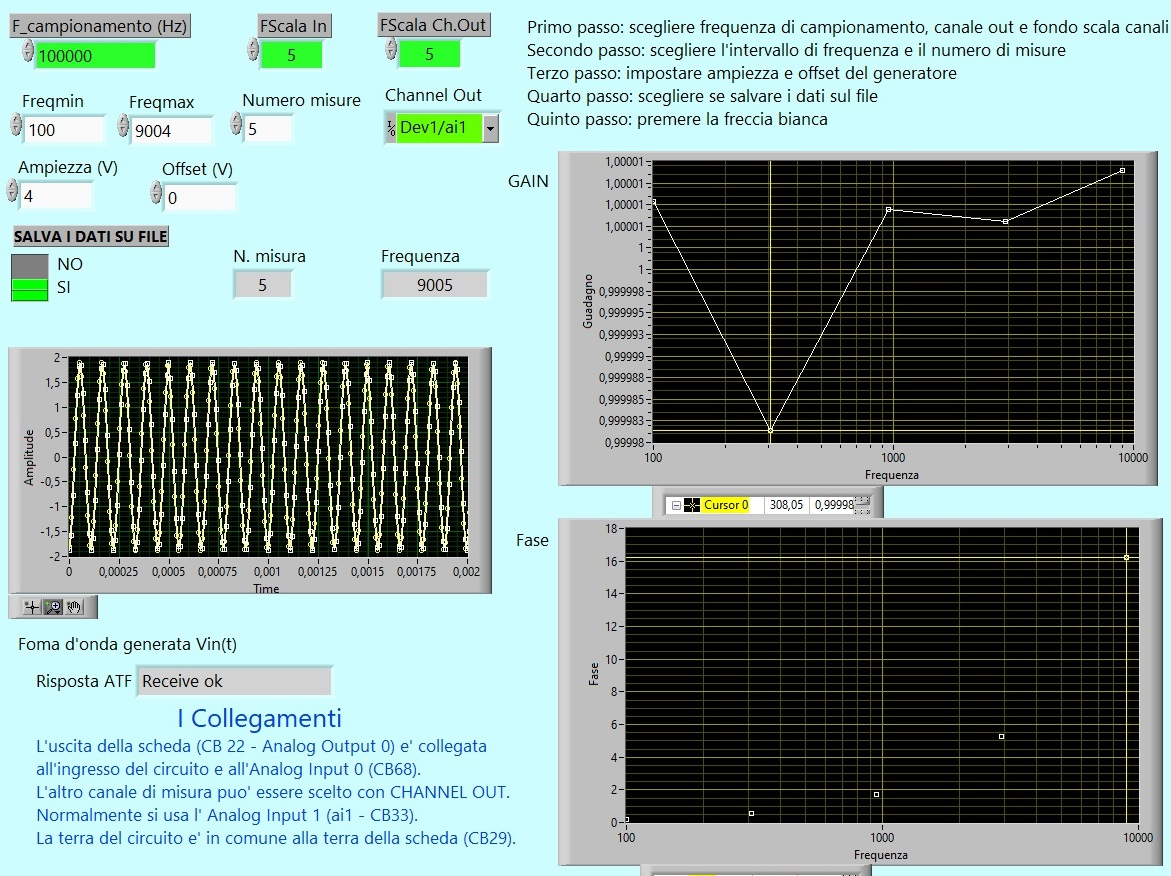
\includegraphics[width=12cm]{settimana_2/immagini/corto_1.jpg}
    \centering
\end{figure}

\LogMark{Acquisizione 2}{17:18}
Facciamo una seconda acquisizione della tensione ai capi del cortocircuito. All'interno della presente è adottato un numero di misure pari a 50. Riportiamo di seguito cosa vediamo sull'interfaccia:
\begin{figure}[H]
\caption{}
    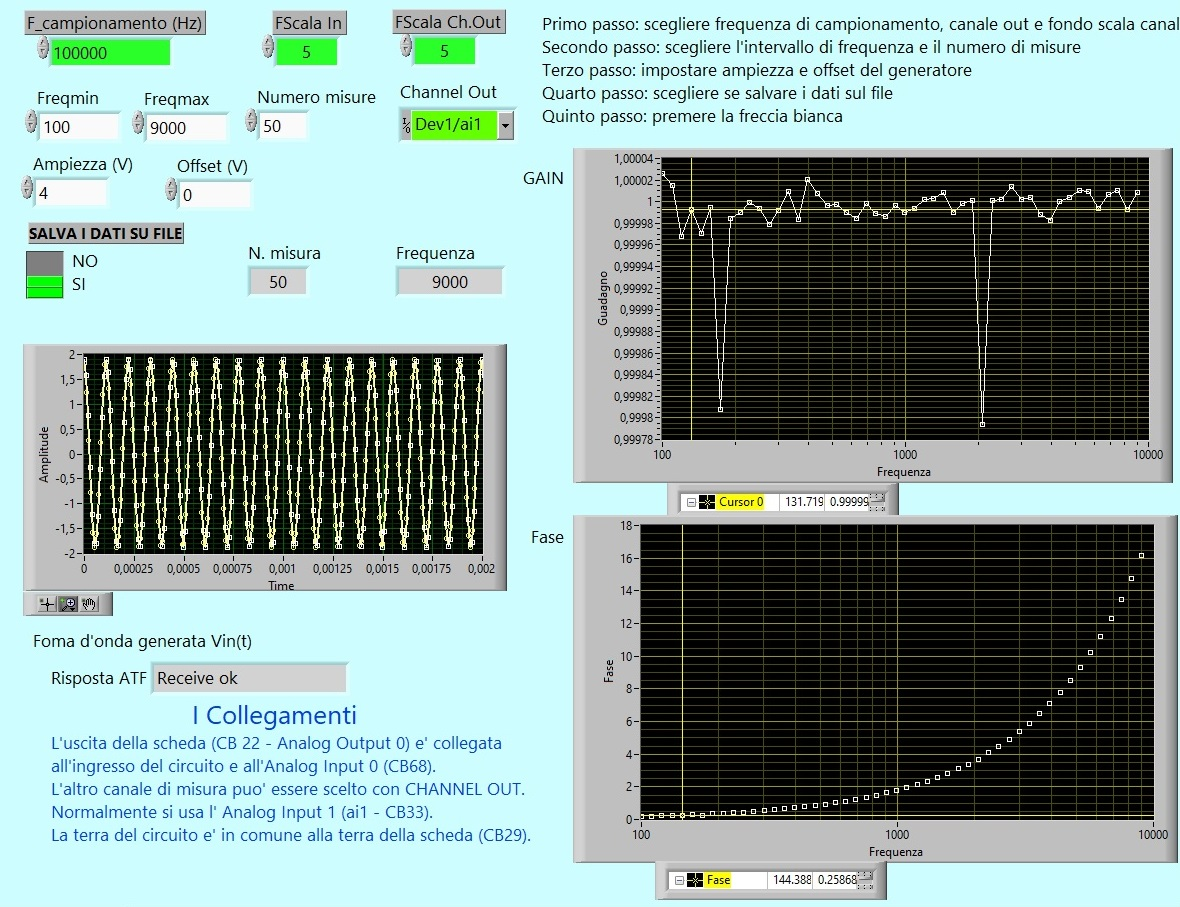
\includegraphics[width=12cm]{settimana_2/immagini/corto_2.jpg}
    \centering
\end{figure}
All'interno del grafico relativo all'ampiezza, notiamo la presenza di due picchi molto accentuati. Per comprenderne la natura, vogliamo fare un confronto con altre acquisizioni.
Osserviamo un andamento non costante (crescente) all'interno del grafico della differenza di fase. Idealmente, essendo la differenza di potenziale ai capi di un cortocircuito quella che misuriamo, il segnale in ingresso dovrebbe risultare identico in ampiezza e fase a quello in uscita. Tuttavia, come possiamo osservare, solo l'andamento dell'ampiezza (fatta eccezione per i due picchi) rispechia approssimativamente l'andamento qualitativo aspettato. Sospettiamo che tale scostamento dall'atteso sia dovuto al fatto che i segnali di ingresso e di uscita sono misurati in due istanti diversi, distanziati normalmente di un intervallo dell'odine (poco superiore) del tempo di digitalizzazione. 

\Nota{
    I dati acquisiti sono disponibili nella cartella \text{"settimana\_2"}
}

\TODO{
    Studiare meglio le caratteristiche della lettura analogica
}

\LogMark{Acquisizione 3}{17:23}
Realizziamo la terza presa, cambiando il solo offset (per vedere se influisce sui risultati), che poniamo pari a 0.5 V. Di seguito riporto i grafici risultanti:
\begin{figure}[H]
\caption{}
    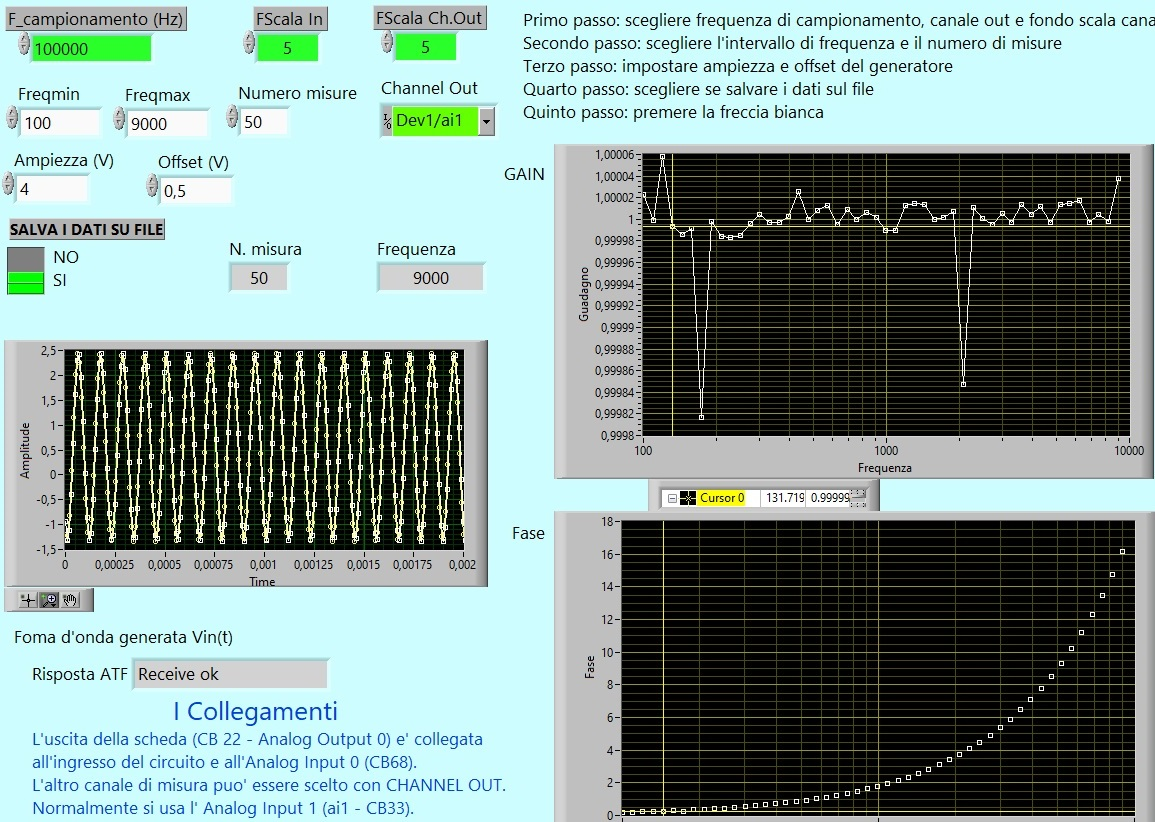
\includegraphics[width=12cm]{settimana_2/immagini/corto_3.jpg}
    \centering
\end{figure}
Vi sono due picchi accentuati che si discostano dall'andamento costante approssimativamente alle stesse frequenze rispetto al caso precedente ($\approx{170Hz}$ e $\approx{2,07kHz}$). Conseguentemente, potremo pensare che questa eventualità sia dovuta a degli effetti che abbiamo a che vedere con le modalità di acquisizione ed analisi dei dati da parte della scheda e del VI dedicato.

\TODO{
    Capire come il VI calcola guadagno e sfasamento e \sout{come la frequenza può influire su di esso} (l'andamento con la frequenza è stato analizzato il 5/10/20).
}

\LogMark{Acquisizione 4}{17:30}
Abbiamo ampliato il range delle frequenze spaziate così da poter valutare meglio gli effetti di essa sull'andamento degli sfasamenti. Osservando l'andamento di questi dal grafico di anteprima, l'andamento sembra simile a quelli precedenti, che suggerisce una dipendenza lineare con la frequenza.
%Aumentiamo da 9 000 a 20 000 e minima da 100 a 50 per vedere se cambia quella cosa sullo sfasamento

\begin{figure}[H]
\caption{}
    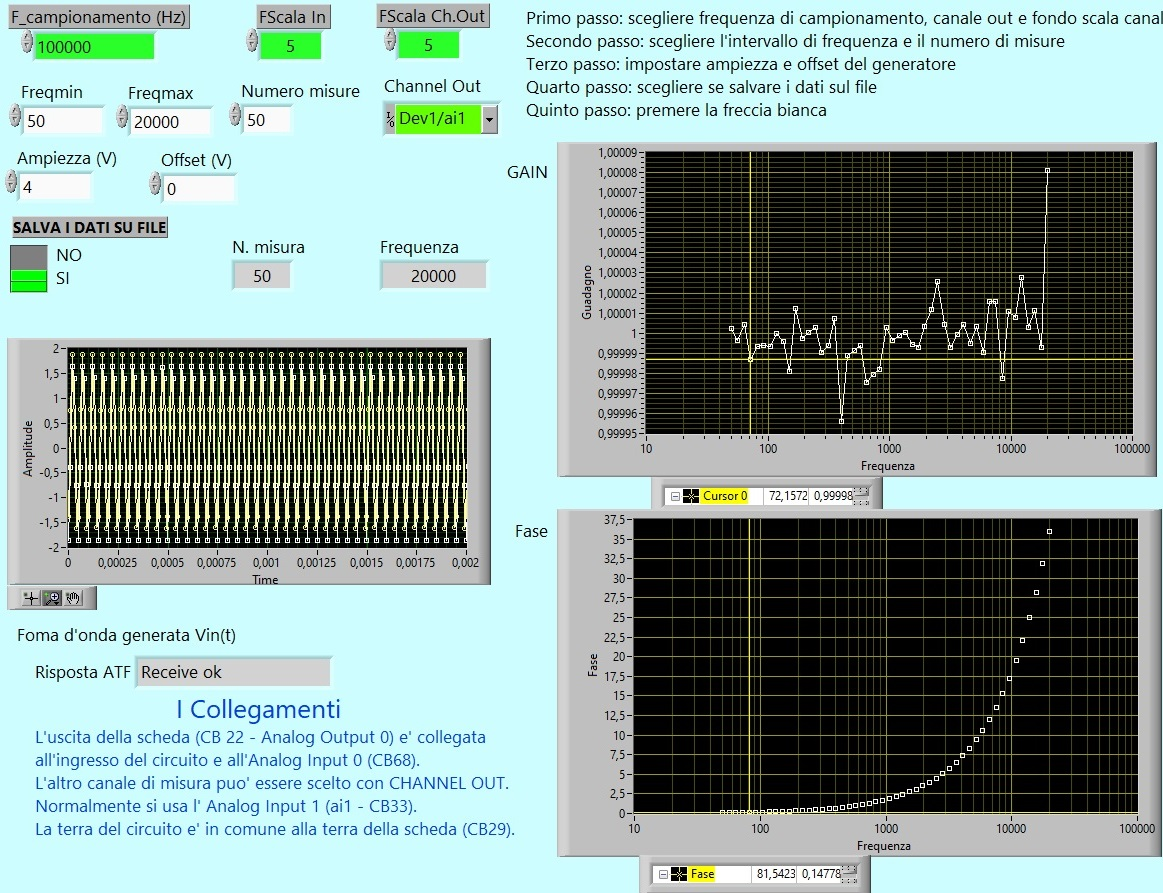
\includegraphics[width=12cm]{settimana_2/immagini/corto_4.jpg}
    \centering
\end{figure}

\Nota{
    I picchi potrebbero essere una sorta di battimento.
}

\LogMark{Acquisizione 5}{17:35}
Abbiamo raddoppiato la frequenza di campionamento (20kHz) per comprendere come tale parametro influisca sullo sfasamento. Dai grafici presentati essi risultano circa dimezzati.

Queste osservazioni si spiegerebbero se le misure di due canali non fossero esattamente contemporanee, ma sfasate di una certa quantità dipendente dalla frequenza di campionamento.

\begin{figure}[H]
\caption{}
    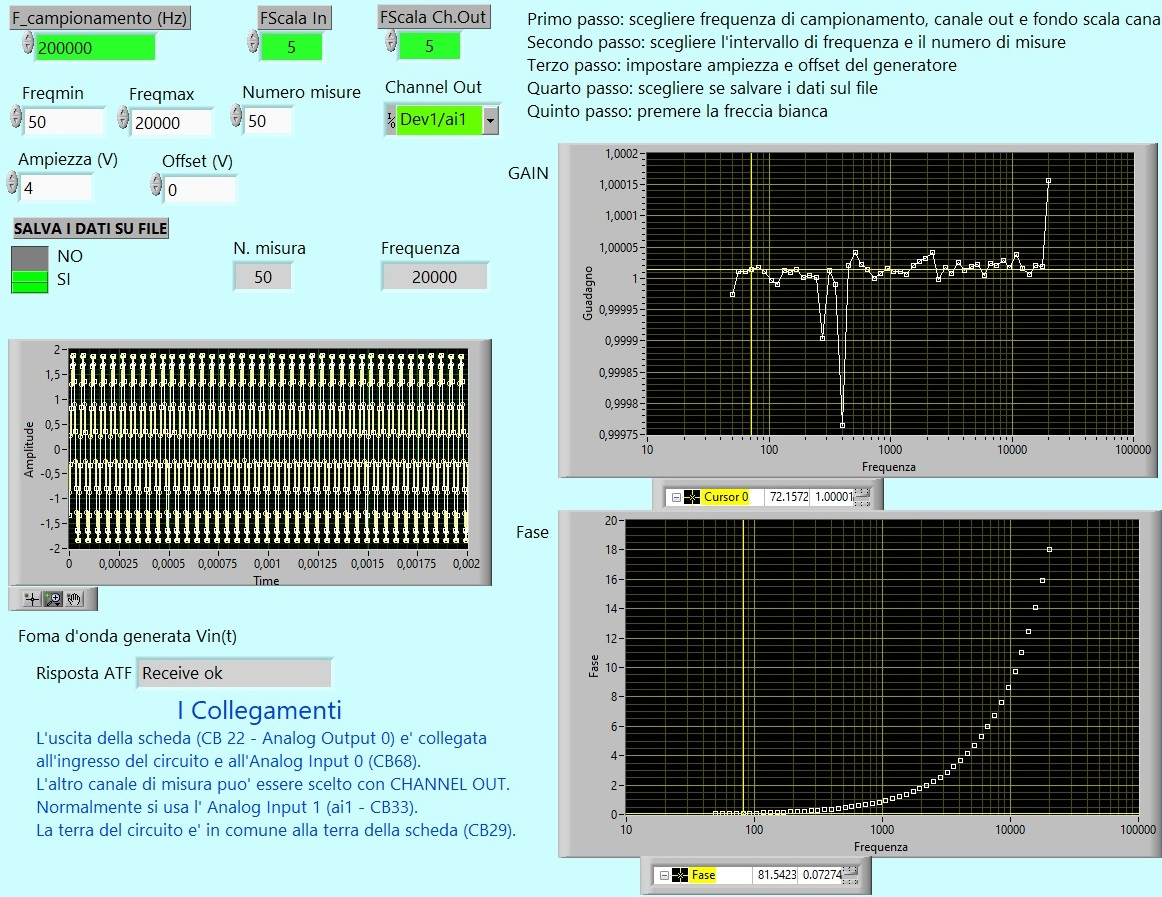
\includegraphics[width=12cm]{settimana_2/immagini/corto_5.jpg}
    \centering
\end{figure}

\Avvertimento{
    Lo sfasamento introdotto dal sistema di lettura diminuisce con la frequenza di campionamento e aumenta con la frequenza.
}

\LogMark{Acquisizione 6}{17:43}
Variamo l'ampiezza a 2 V, lasciando gli altri parametri invariati.
L'andamento risulta essere simile a quello dell'acquisizione precedente. La sola differenza visibile connsiste nella presenza di una maggiore variazione dei guadagni attorno l'unità. Le variazioni del guadagno potrebbero essere dovute alla presenza del rumore.

\begin{figure}[H]
\caption{}
    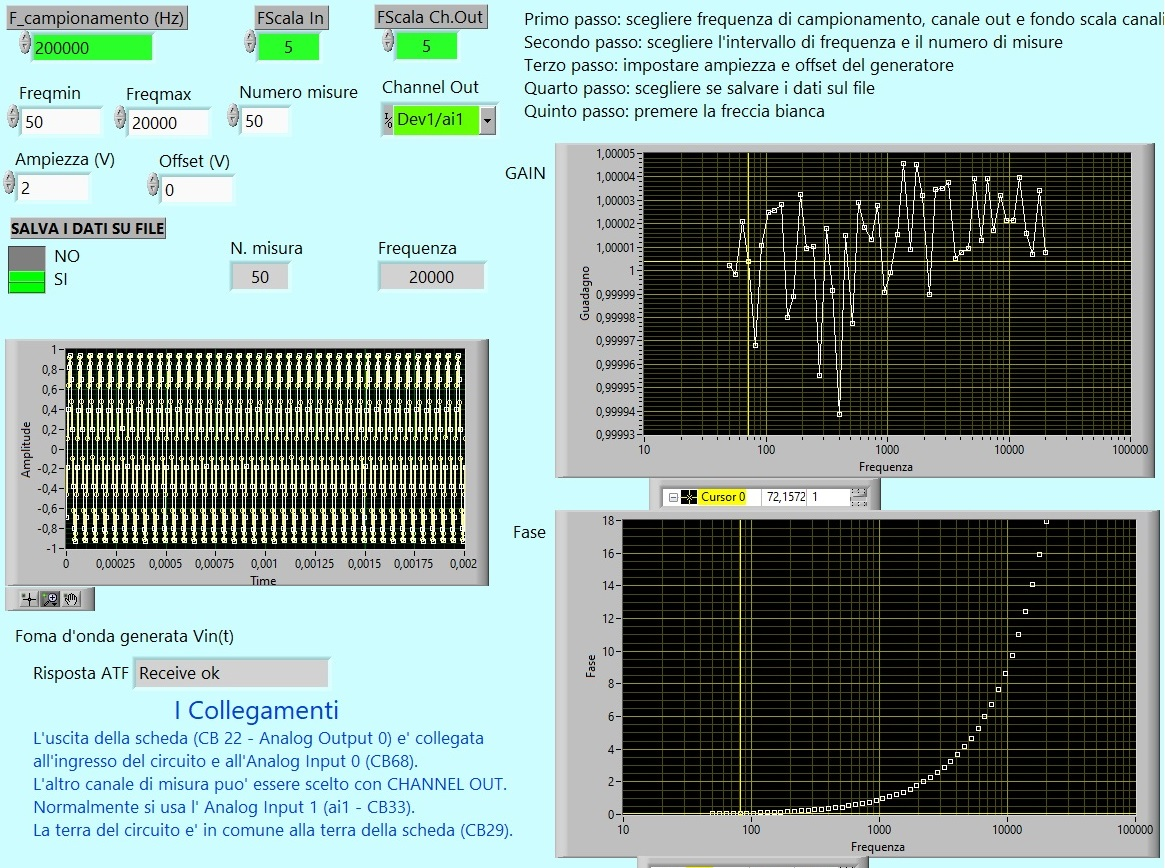
\includegraphics[width=12cm]{settimana_2/immagini/corto_6.jpg}
    \centering
\end{figure}

\NewSection{Filtro CRRC}
\Orario{17:47}
Ora impostiamo quale canale di uscita il Dev1/ai2. Tale porta è collegata all'uscita di un filtro CRRC. I valori nominali delle resistenze e delle capacità sono riportati all'interno del presente schema, realizzato in TINA:
\begin{figure}[H]
\caption{}
    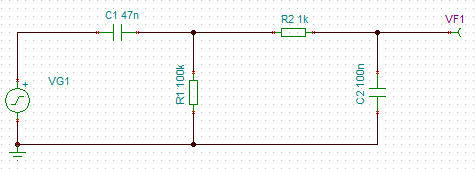
\includegraphics[width=8cm]{settimana_2/immagini/ImmagineCRRC.png}
    \centering
\end{figure}

Attraverso il comando dell'"AC Transfer Characteristic" vediamo cosa ci aspettiamo dai diagrammi di Bode per questo circuito, variando la frequenza da 10 Hz a 20 kHz:
\begin{figure}[H]
\caption{}
    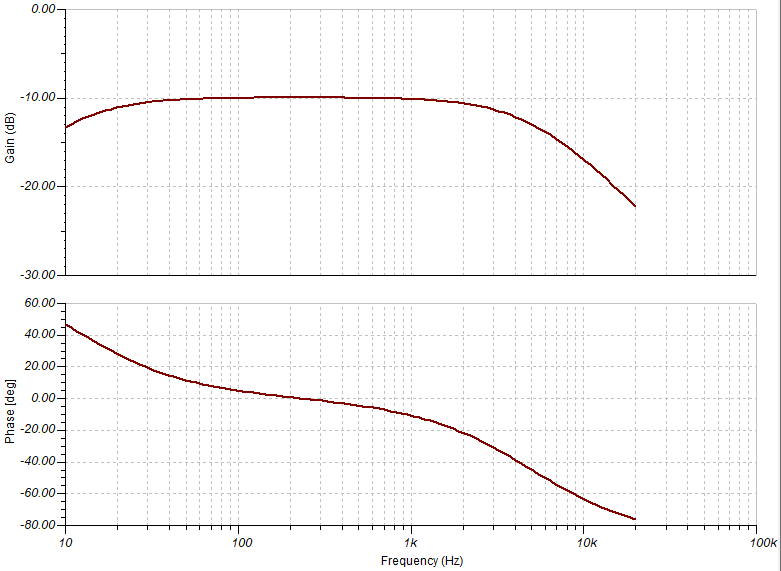
\includegraphics[width=8cm]{settimana_2/immagini/ImmagineCRRCBodeatteso.png}
    \centering
\end{figure}

\LogMark{Acquisizione di prova}{17:48}
Impostiamo il numero di misure a 10 per verificare il corretto funzionamento dell'acquisizione.

\begin{figure}[H]
\caption{}
    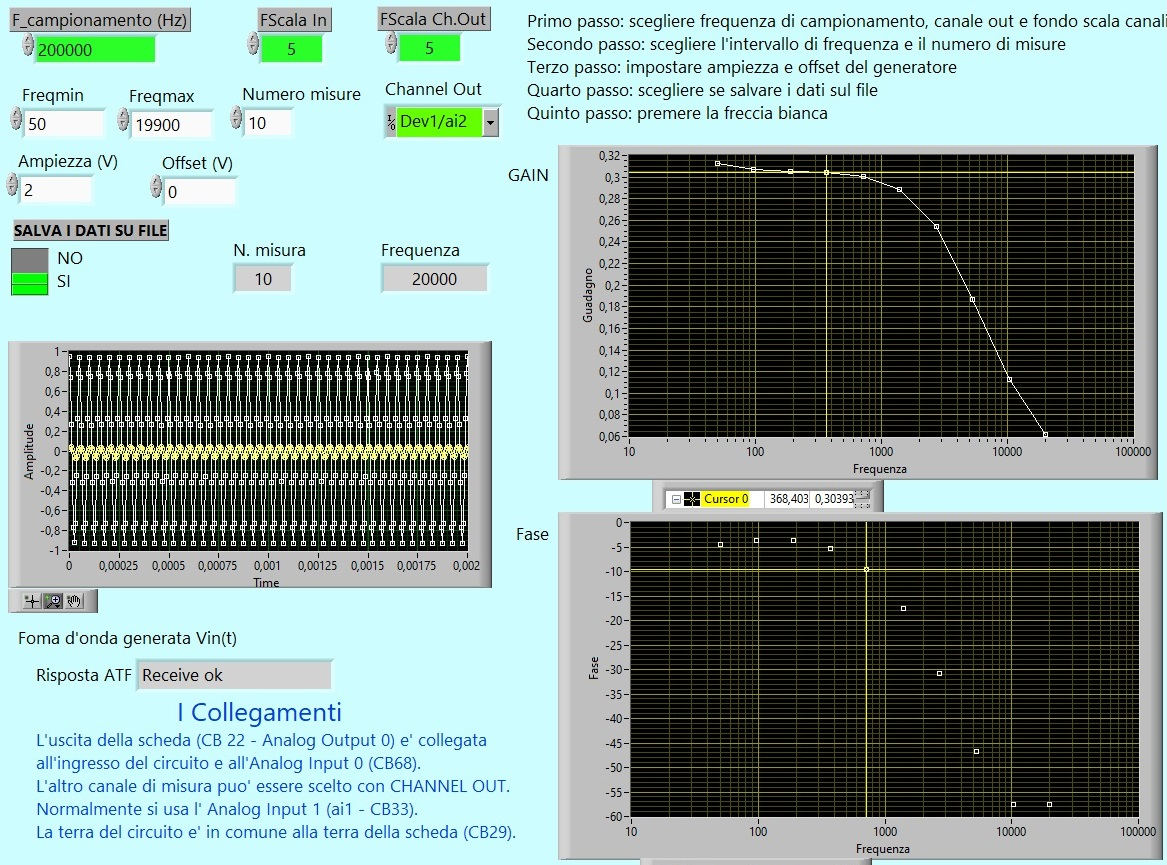
\includegraphics[width=12cm]{settimana_2/immagini/CRRC_1.jpg}
    \centering
\end{figure}

\LogMark{Acquisizione 2}{17:55}
Lanciamo un'altra acquisizione lasciando invariati tutti i parametri fatta eccezione del numero di misure, posto pari a 50. In tal modo, l'andamento dei dati risulterà più dettagliato e significativo.


\begin{figure}[H]
\caption{}
    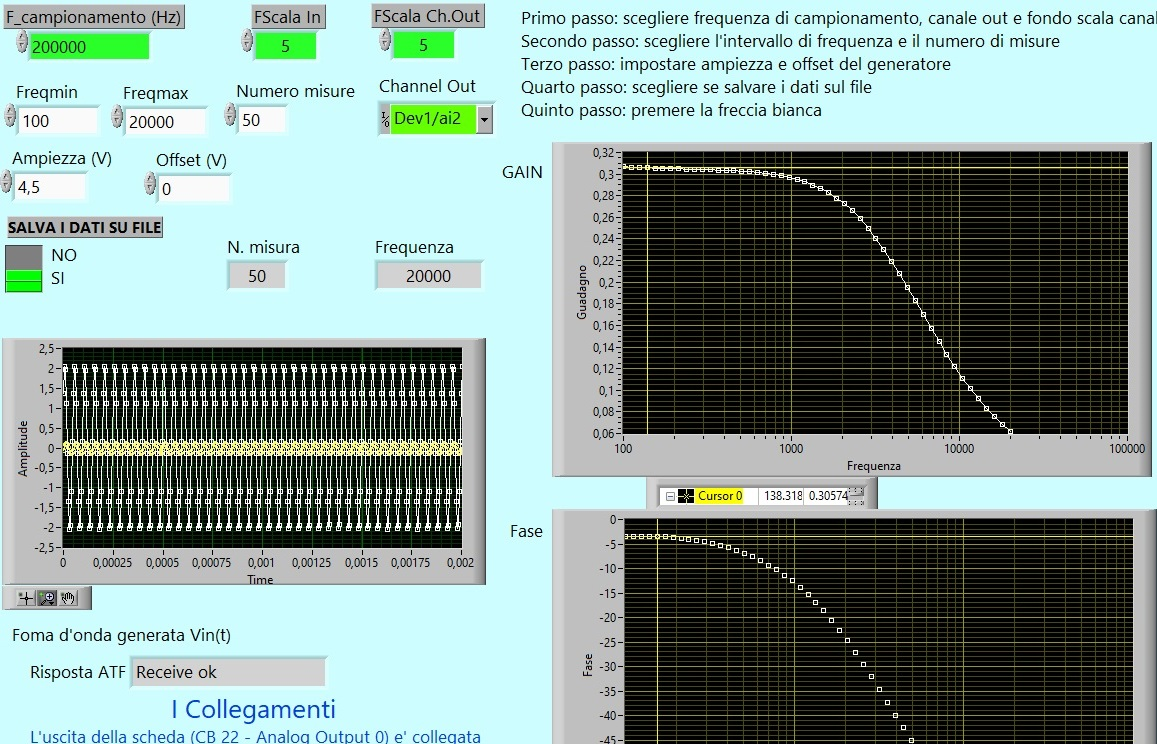
\includegraphics[width=12cm]{settimana_2/immagini/CRRC_2.jpg}
    \centering
\end{figure}

Notiamo che a basse frequenze il guadagno aumenta, al contrario di quello che ci saremmo aspettati. Pensiamo che questo effetto sia dovuto ad effetti difficilmente stimabili dovuti al sistema di acquisizione. Di conseguenza nelle acquisizioni successive non useremo frequenza più basse di 50Hz, al fine di evitare di registrare dati affetti da problematiche del sistema di acquisizione.

Osserviamo che l'andamento dello sfasamento risulta essere crescente nell'ultimo tratto. Ciò è presumibilmente dovuto alla differenza temporale fra le acquisizioni dei due canali, la quale diviene sempre meno trascurabile (divenendo sempre più paragonabile al periodo dell'onda in ingresso) all'aumentare della frequenza.

\Nota{Parleremo meglio di come il sample rate sia legato alla curvatura dello sfasamento in seguito}

\Nota{
    In un secondo momento abbiamo capito che è possibile acquisire correttamente alle frequenze basse, a patto di diminuire adeguatamente il sample rate. Vedere le note del giorno 02/10/2020.
}

\Nota{
    Questa immagine e le successive (di questa giornata) sono state salvate in modo erroneo e purtoppo non si vedono bene i grafici degli sfasamenti.
}

\LogMark{Acquisizione 3}{18:00}
Lanciamo un'altra acquisizione, in cui stavolta il range di frequenze spazia da 1 kHz a 50 kHz.

\begin{figure}[H]
\caption{}
    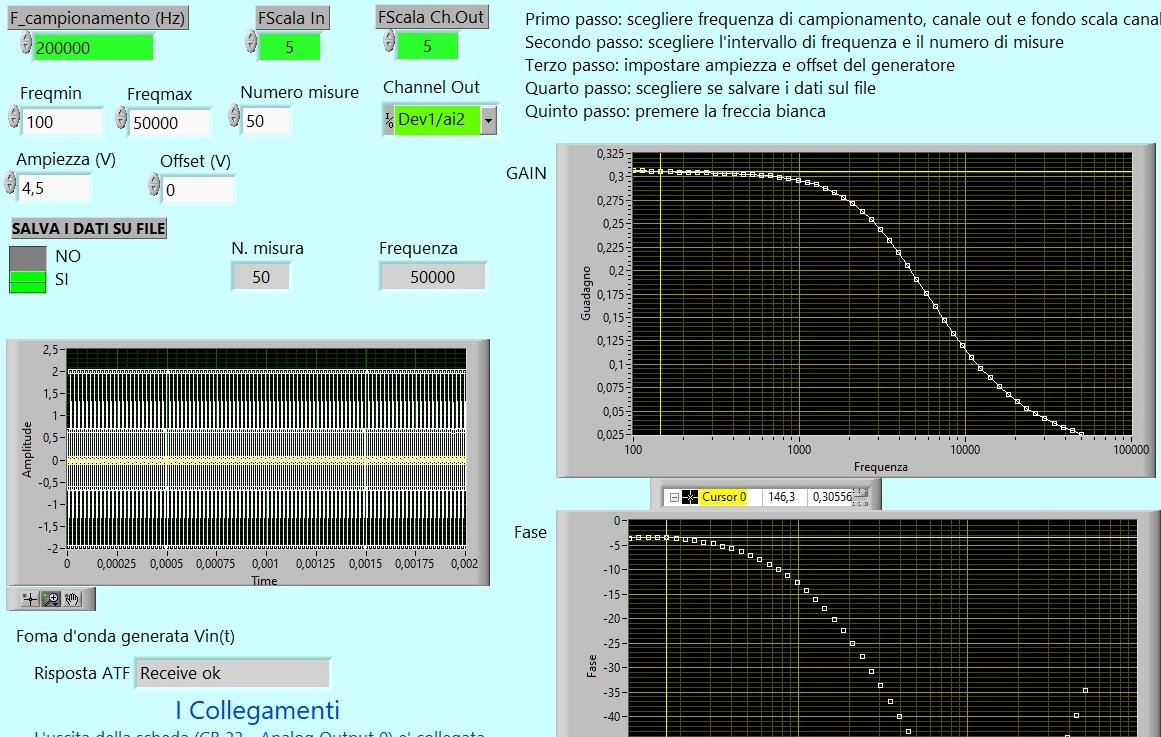
\includegraphics[width=12cm]{settimana_2/immagini/CRRC_3.jpg}
    \centering
\end{figure}

In questo set di dati, l'andamento crescente dell'ultimo tratto dello sfasamento si nota in maniera più accentuata.

\LogMark{Acquisizione 4}{18:03}
Lanciamo una nuova acquisizione, riempostando la frequenza massima a 20 kHz e l'ampiezza a 2 V, per osservare cosa avviene al segnale acquisito al variare della scala di tensione.

\begin{figure}[H]
\caption{}
    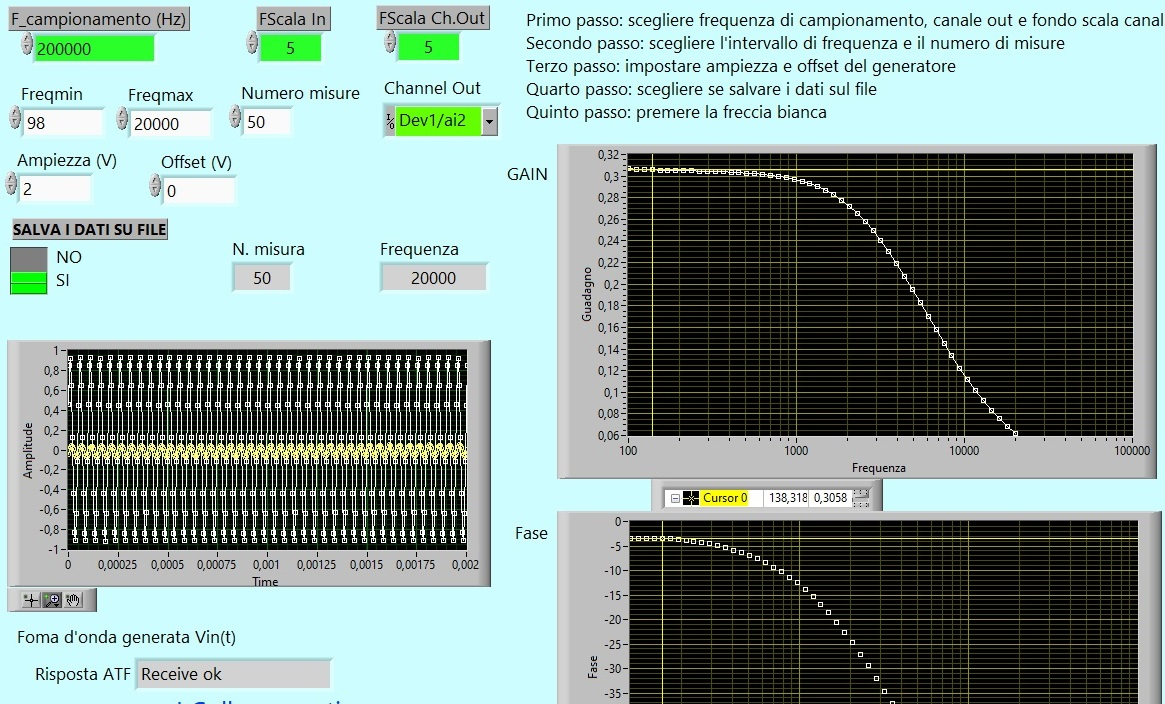
\includegraphics[width=12cm]{settimana_2/immagini/CRRC_4.jpg}
    \centering
\end{figure}
Gli andamenti del guadagno e dello sfasamento non risultano differire significativamente rispetto all'acquisizione con ampiezza maggiore e opari gli altri parametri.

\LogMark{Acquisizione 5}{18:06}
Facciamo una nuova acquisizione, lasciando invariati tutti i parametri della oprecedente fuorchè l'offset, posto a 2V.

\begin{figure}[H]
\caption{}
    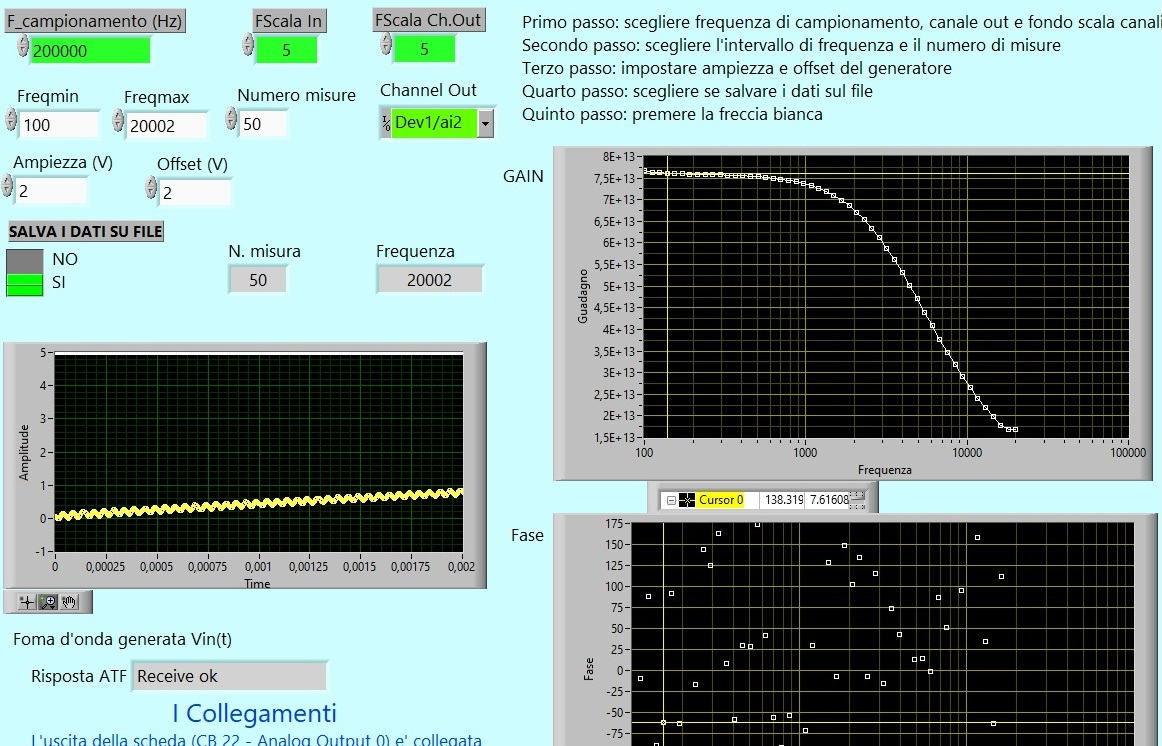
\includegraphics[width=12cm]{settimana_2/immagini/CRRC_5.jpg}
    \centering
\end{figure}

Osserviamo che l'andamento dello sfasamento non risulta affatto simile a quello atteso, più precisamente i valori sembrano essere completamente scorrelati, come se fosse rumore. All'interno del grafico del guadagno, inoltre, la scala delle ordinate risulta essere amplificata così da riosultare dell'ordine di $10^{13}$, cosa assolutamente insensata per un guadagno di un attenuatore con soli elementi passivi (fatta eccezione del generatore di tensione, che però possiamo supporre influire trascurabilmente, anche alla luce dei dati delle acquisizioni precedenti). Infine possiamo osservare dal grafico a sinistra che l'onda in ingresso sembra essere al di fuori del fondo scala. Tuttavia essa dovrebbe spaziare fra 0 e 4 V per i parametri adottati ed abbiamo usato un fondo scala di 5 V per il segnale in ingresso. 
Al momento non ci è chiaro il motivo dei nostri risultati. Cercheremo dunque di analizzare il presente fenomeno in altre acquisizioni successive.

\LogMark{Acquisizione 6}{18:10}
Eseguiamo una prova con gli stessi parametri per osservare se vi è stata o meno una lettura erronea nel caso precedente.

\begin{figure}[H]
\caption{}
    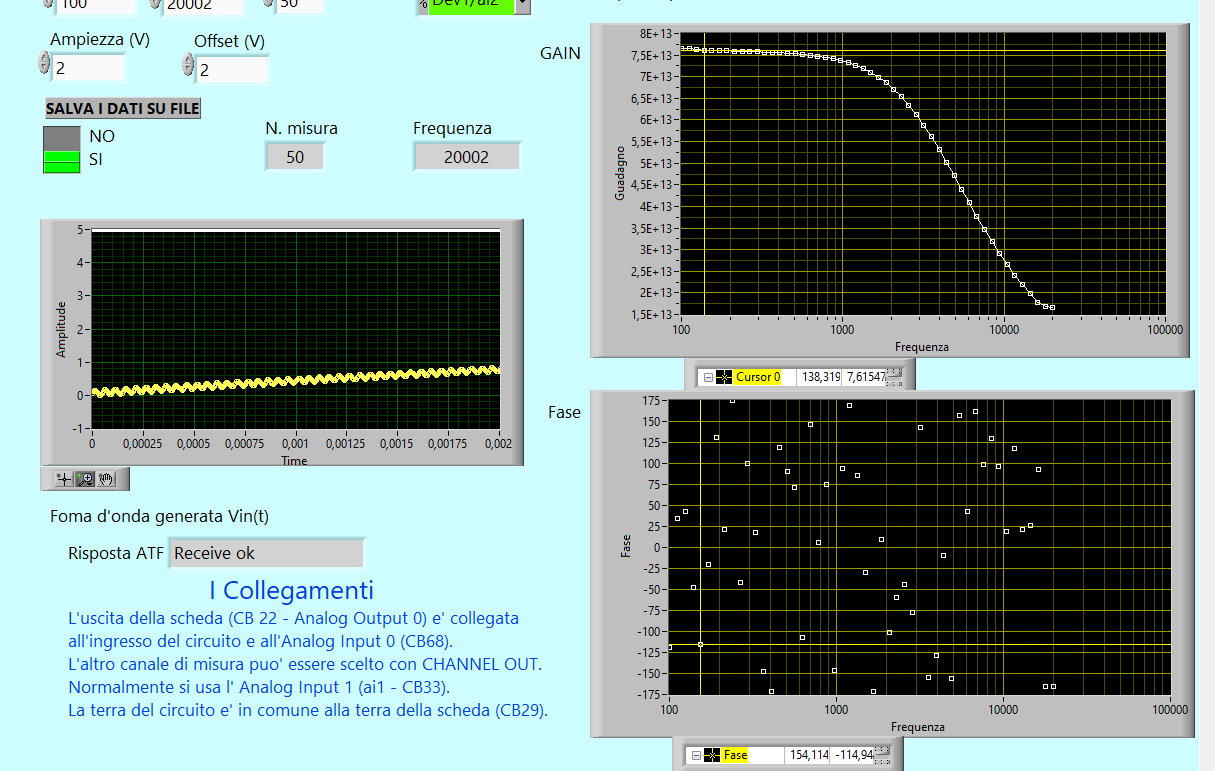
\includegraphics[width=12cm]{settimana_2/immagini/ACQUIS6pomeriggiomartediritagliatax.png}
    \centering
\end{figure}

I risultati non presentano differenze rilevanti rispetto ai ai precedenti. 

\LogMark{Acquisizione 7}{18:20}
Riproviamo con un offset più piccolo (0.5V) per vedere se i risultati risultano essere migliori con questa differenza.

\begin{figure}[H]
\caption{}
    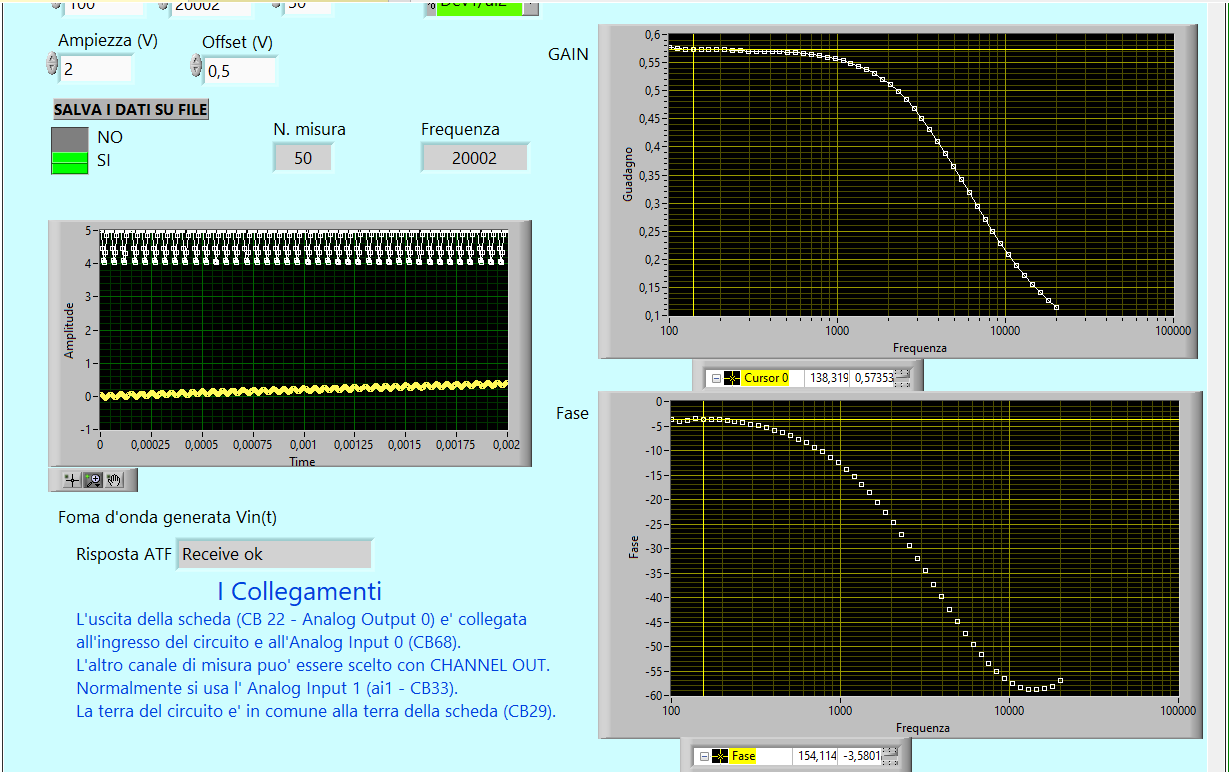
\includegraphics[width=12cm]{settimana_2/immagini/ACQUIS7pomeriggiomartediritagliatax.png}
    \centering
\end{figure}

Osserviamo che in questo caso, la differenza di fase risulta avere un andamento migliore rispetto ai due casi precedenti (in relazione al confronto con quello atteso). Tuttavia il guadagno risulta amplificato di un certo fattore rispetto al caso di assenza di offset (rimanendo pur sempre dell'ordine di $0.1 \sim 1$). Infine, gli andamenti dell'onda in ingresso e di quella in uscita (rappresentati nel grafico a sinistra) non risultano affatto simili a quelli che ci aspetteremo coi parametri selezionati: l'onda ingresso sembra avere offset pari a 5 V anzichè a 0.5 V. L'onda risulta perciò segata a metà. Ciò spiegherebbe l'esattezza qualitativa degli andamenti nel grafico dell'attenuazione e della differenza di fase ed anche il motivo per cui quantitativamente sono diverse (per un'onda segata la funzione di trasferimento andrebbe applicata diversamente (alle componenti armoniche, ricavabili attraverso la trasformata discreta di Fourier) e quindi è sbagliata la stima dell'ampiezza in ingresso).

\Avvertimento{
    \Orario{18:22}Pensiamo che ci possa essere qualche problema nel circuito, ad esempio un errore sui riferimenti delle masse (osservare che il grafico di V\textsubscript{out} sembra avere una pendenza positiva in aggiunta al segnale sinusoidale mentre V\textsubscript{in} risulta saturato). Questo comunque non spiegerebbe perchè quando l'offset è a zero non ci siano problemi.
}

\LogMark{Acquisizione 8}{18:37}
Aseguiamo un'altra prova per controllare se sia cambiato qualcosa, riceviamo tuttavia dati simili ai precedenti.

\LogMark{Acquisizione 9}{18:58}
Su consiglio del professore, riporviamo con una frequenza diversa (100 kHz). Potremmo infatti stare ricevendo risultati errati a causa di sample rate troppo elevati. Visivamente non troviamo tuttavia alcun cambiamento significativo.

%%%%%%%%%%%%%%%%%%%%%%%%%%%%%%%%%%%%%%%%
%%%%%%%%%%%%  NEW DAY %%%%%%%%%%%%%%%%%%
%%%%%%%%%%%%%%%%%%%%%%%%%%%%%%%%%%%%%%%%

\NewDay{Acquisizioni con filtro RCCR}{01/10/2020}
All'interno di questo pomeriggio analizzeremo i diagrammi di Bode ottenuti attraverso un circuito RCCR, realizzato scambiando i filtri passa-basso e passa-alto che componevano il circuito CRRC precedentemente analizzato.

\Orario{15:10}
Entriamo nel portale adottato previamente per le acquisizioni col filtro CRRC: \textcolor{airforceblue}{\url{http://131.114.11.57:8000/BODE1.html}}.

\Nota{
    Per errore, parte delle schermate catturate sono state tagliate (il grafico degli sfasamenti è solo parzialmente visibile). Comunque le osservazioni fatte sul posto sono state descritte nelle varie entry. Tutti i dati sono stati salvati e caricati sulla repository e verranno comunque analizzati successivamente.
}

\LogMark{Simulazione del circuito con TINA}{15.15}
Il nostro scopo è analizzare il guadagno e lo sfasamento in funzione della frequenza. 
Come operazione preliminare, andiamo su TINA per simulare il circuito e osservare la risposta ideale che ci aspetteremo di ottenere coi parametri dati nella scheda della settimana 2. I valori nominali risultano essere: $C_1 = 47$ $nF$, $C_2 = 100$ $nF$, $R_1 = 100$ $k\Omega$ e $R_2 = 1$ $k\Omega$.

\Nota{Le resistenze e le capacità reali potrebbero non essere affatto quelle nominali. Le resistenze e le capacità nominali prosposte sono da considerarsi valide solo per fini approssimativi/qualitativi}

Riportiamo di seguito lo schema del circuito e i diagrammi di Bode ottenuti con il comando AC Transfer Characteristic (abbiamo adottato un range di frequenze che spazia da 10 Hz a 9 kHz):

\begin{figure}[H]
\caption{}
    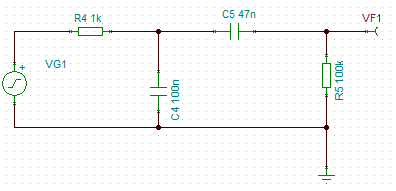
\includegraphics[width=7cm]{settimana_2/immagini/ImmagineRCCR.png}
    \centering
\end{figure}


\begin{figure}[H]
\caption{}
    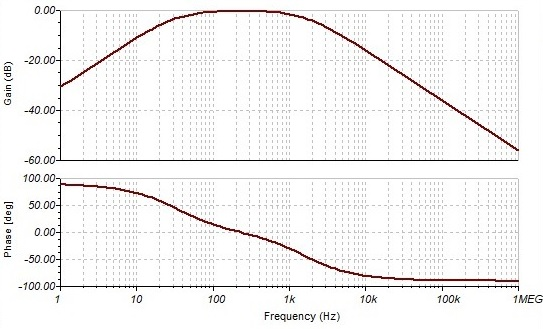
\includegraphics[width=7cm]{settimana_2/immagini/RCCR_tina_transfer.jpg}
    \centering
\end{figure}

\LogMark{Acquisizione preliminare}{15.37}
Realizziamo una prima acquisizione con numero di punti pari a 10 ai fini di verificare il funzionamento dell'acquisizione. La frequenza minima e massima adottata risultano rispettivamente pari a 10 Hz e 9 kHz.

\begin{figure}[H]
\caption{}
    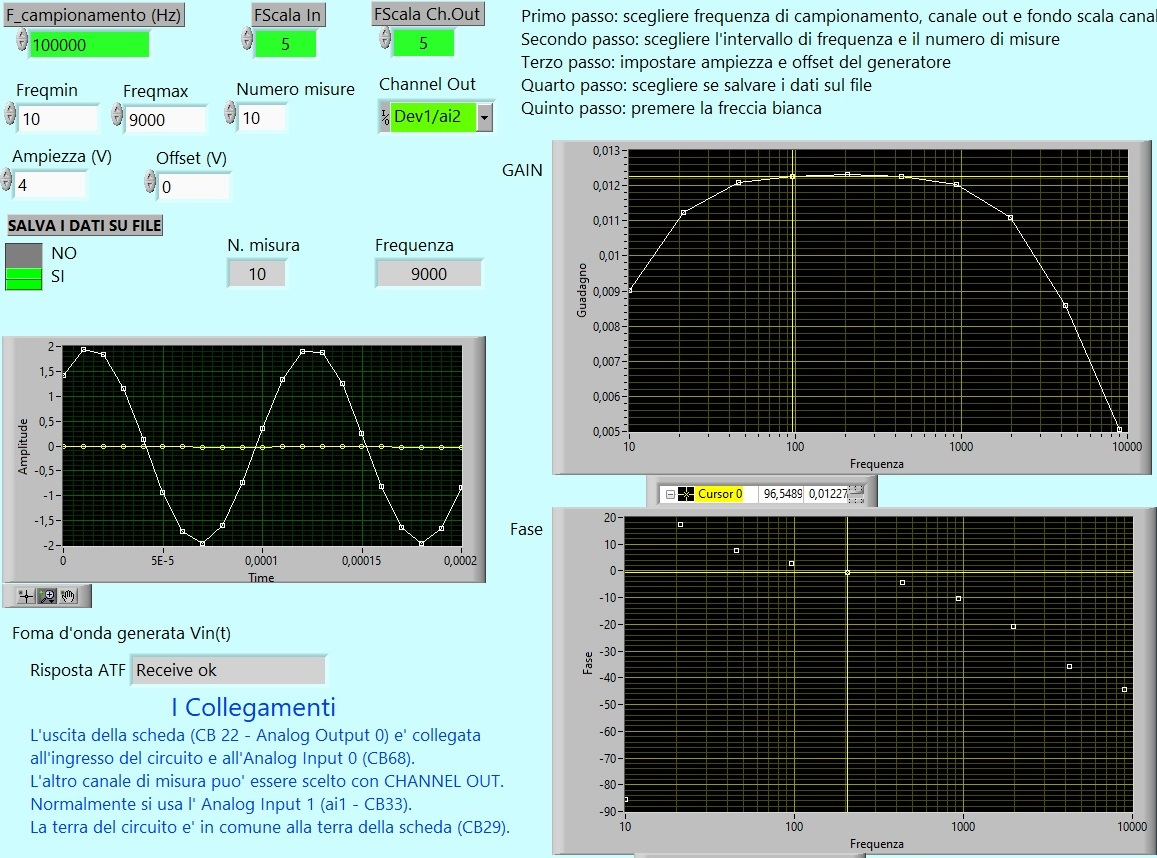
\includegraphics[width=12cm]{settimana_2/immagini/rccr_1.jpg}
    \centering
\end{figure}

Gli andamenti risultano qualitativamente simili a quelli aspettati.

\LogMark{Acquisizione 2}{15.41}
Lasciando invariati gli altri parametri, adottiamo una frequenza massima ed un numero di misure rispettivamente pari a 20 kHz e 100.

\begin{figure}[H]
\caption{}
    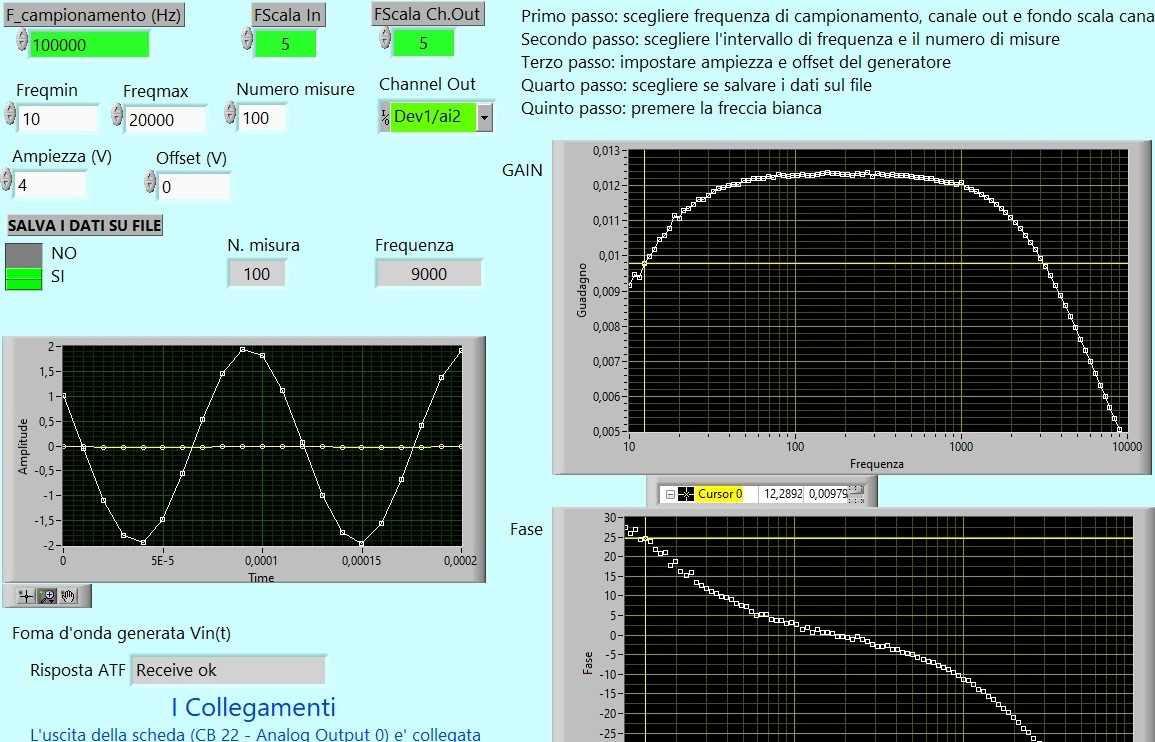
\includegraphics[width=12cm]{settimana_2/immagini/rccr_2.jpg}
    \centering
\end{figure}

Gli andamenti risultano qualitativamente simili agli aspettati. Tuttavia, il massimo del guadagno risulta essere inferiore rispetto a quello riscontrato attraverso la simulazione effettuata con TINA. Ciò potrebbe essere dovuto al fatto che sono stati forniti delle resistenze e capacità che potrebbero differire (pur rimanendo dello stesso ordine) da quelli nominali. In sezioni successive, analizzeremo più in dettaglio questo fattore.

\LogMark{Acquisizione 3}{15.42}
Per indagare sulla possibilità di acquisire con una frequenza maggiore, adottiamo un sampling rate di 200 kHz. All'interno delle nostre acquisizione, è possibile infatti superare il range consigliato nella scheda senza danneggiarla o causare disagi nell'apparato (essendo la nostra scheda la 6024). Potremo notare che ad una frequenza di campionamento troppo elevata, il guadagno e lo sfasamento ricavati possono risultare alterati, nonostante tale limite sia sicuramente  inferiore ai 1.8 GSa/s nominale per una porta in quanto stiamo usando due canali anziché uno per l'acquisizione.


\begin{figure}[H]
\caption{}
    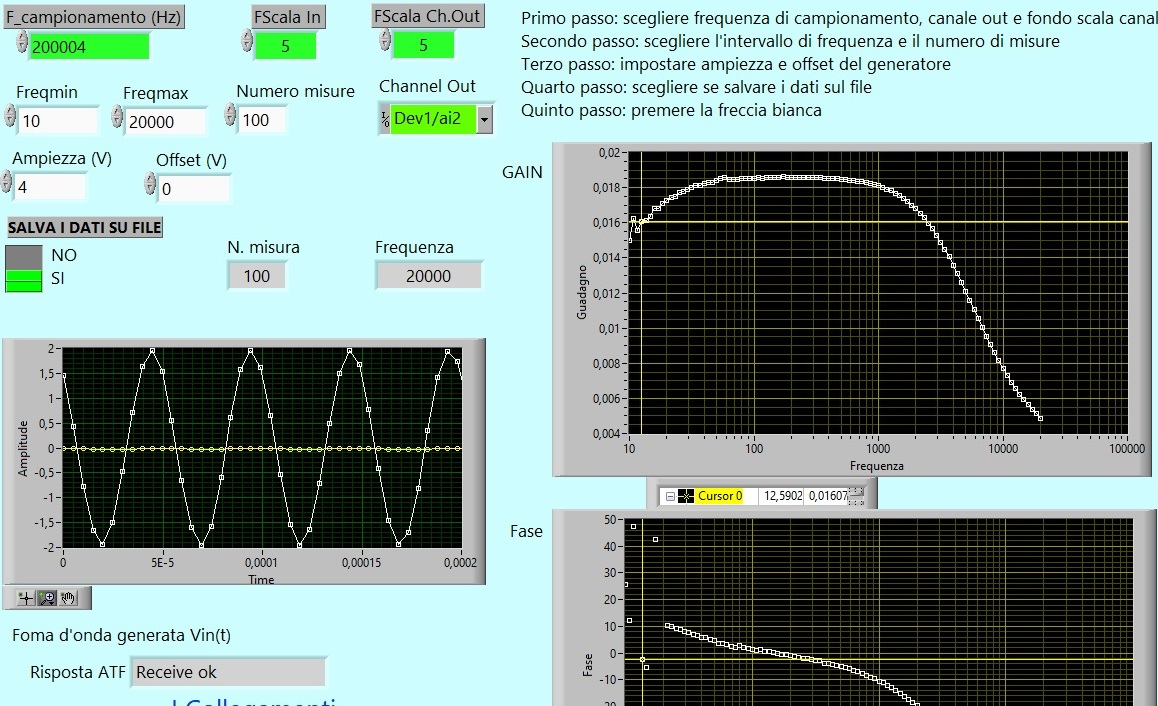
\includegraphics[width=12cm]{settimana_2/immagini/rccr_3.jpg}
    \centering
\end{figure}

Notiamo che per le basse frequenze i valori dei guadagno e sfasamento risultano molto distanti da quelli aspettati. Nelle prove successive useremo dunque una frequenza di campionamento più bassa.

\LogMark{Acquisizione 4}{15.48}
Vogliamo vedere cosa succede quando la forma d'onda risulta sottocampionata. Impostiamo la frequenza massima a 50 kHz ed il sampling rate a 100 kHz. Nel caso di frequenza massima arriveremo, quindi, a due punti per onda, che sicuramente corrisponde ad un sottocampionamento. 

\begin{figure}[H]
\caption{}
    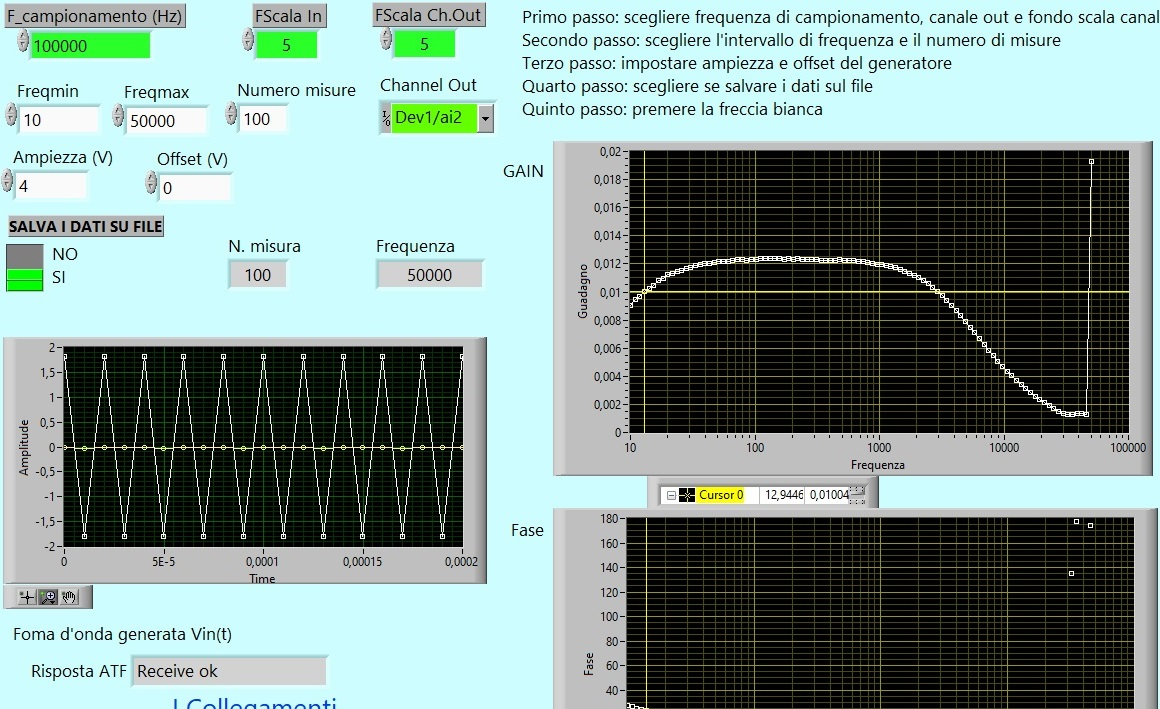
\includegraphics[width=12cm]{settimana_2/immagini/rccr_4.jpg}
    \centering
\end{figure}

Il grafico rispecchia quanto immaginavamo. Come pensavamo, infatti, per alte frequenze si osserva l'effetto di sottocampionamento, che porta dunque a risultati visivamente erronei a paragone con quelli aspettati teoricamente. 

\LogMark{Acquisizione 5}{15.48}
Proviamo a diminuire l'ampiezza in ingresso (1V) per controllare che guadagnio e sfasamento non dipendano da questa variabile.

\begin{figure}[H]
\caption{}
    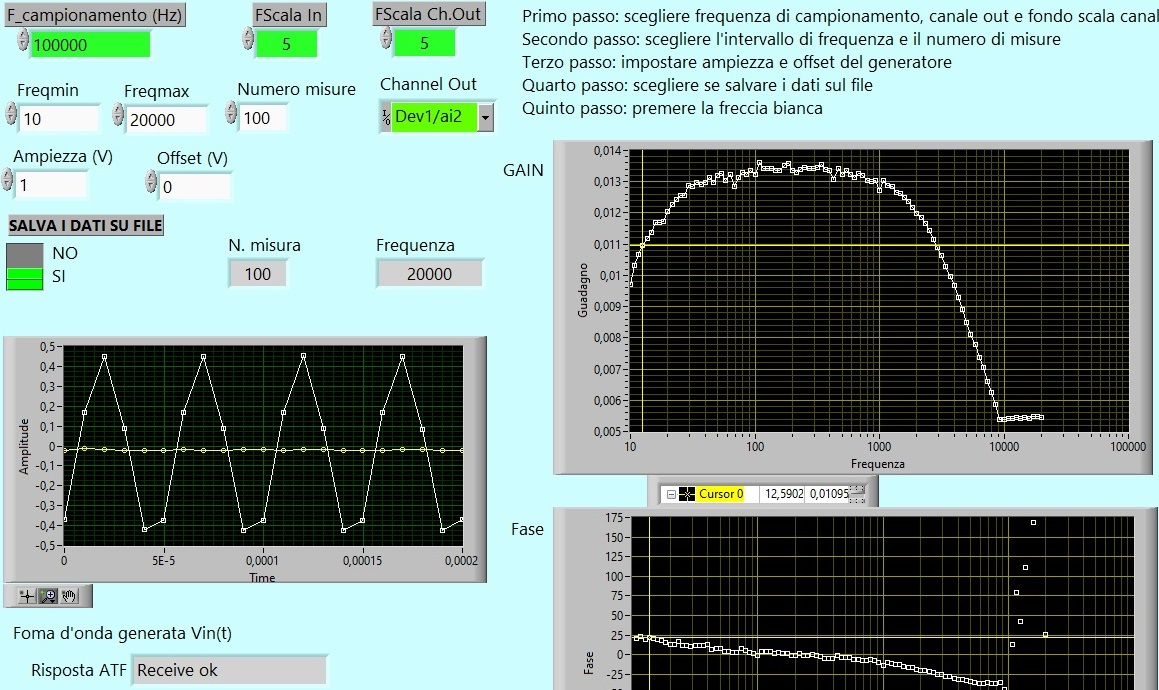
\includegraphics[width=12cm]{settimana_2/immagini/rccr_5.jpg}
    \centering
\end{figure}

Nel grafico l'andamento risulta peculiare (ad alte frequenze si ha un "appaittimento"). Forse è dovuto al fatto che per un ampiezza di questa entità, il segnale su V\textsubscript{out} si confonde col rumore. Facciamo un'altra prova identica per verificare nella prova 6.

\LogMark{Acquisizione 6}{15.53}
Procediamo analogamente a prima.

\begin{figure}[H]
\caption{}
    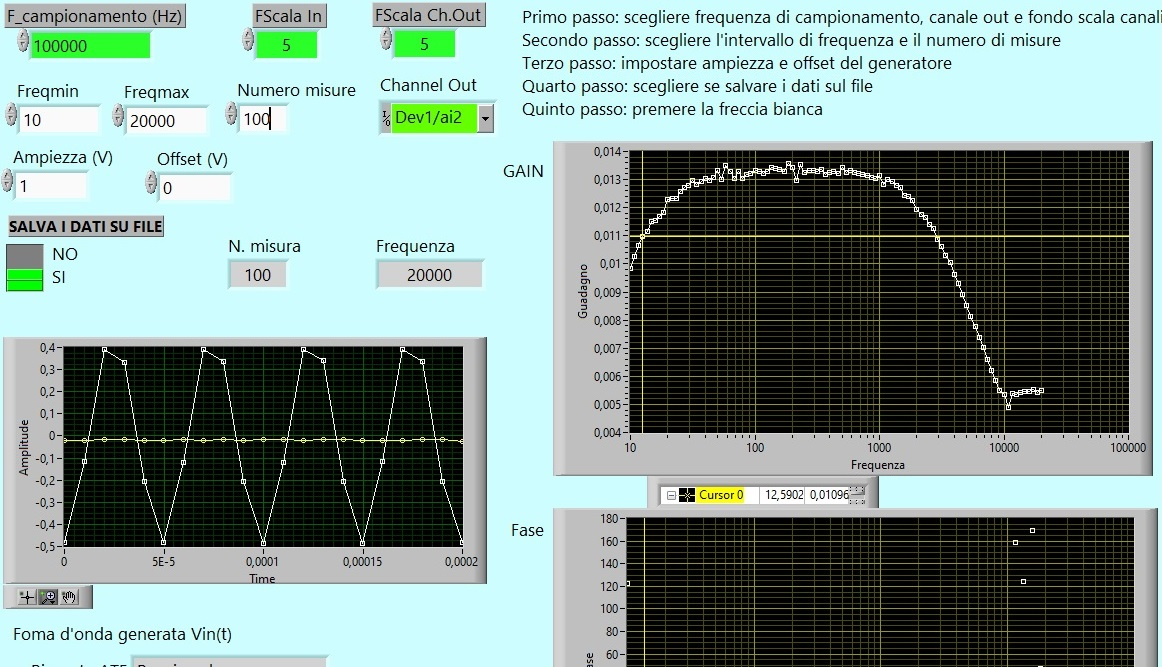
\includegraphics[width=12cm]{settimana_2/immagini/rccr_6.jpg}
    \centering
\end{figure}
Si ottengono risultati analoghi al caso precedente. Quindi possiamo pensare che effettivamente sia presente un fattore di disturbo che influisca sulla qualità dei dati visibilmente.

\LogMark{Acquisizione 7}{15.56}
% forse numeri sono sbaliati
Impostiamo l'ampiezza a 2 V per vedere quanto cambia il rapporto segnale rumore rispetto ai casi relativi a 4 V e a 1 V. 

\begin{figure}[H]
\caption{}
    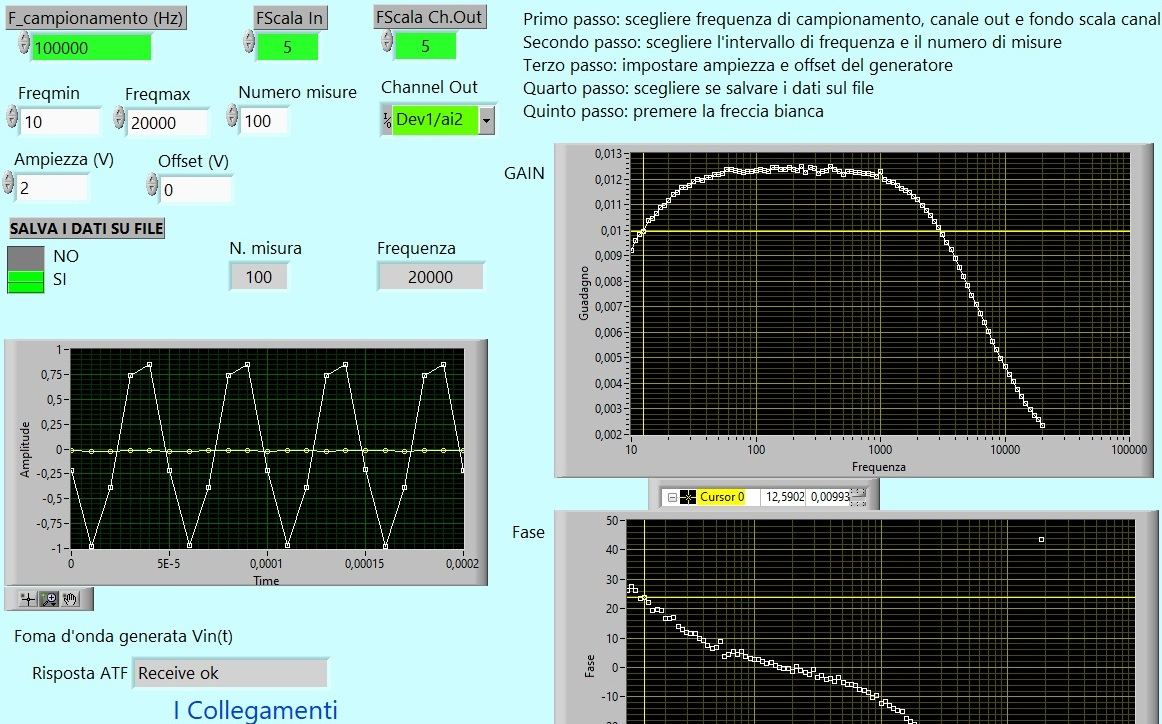
\includegraphics[width=12cm]{settimana_2/immagini/rccr_7.jpg}
    \centering
\end{figure}

Notiamo che ora l'andamento risulta essere più simile a quello aspettato rispetto al caso di ampiezza minore. Tuttavia, specialmente ad alte frequenze, si nota uno scostamento. Questo presumibilmente si ha perchè ad ampiezze piccole il guadagno risulta essere talmente piccolo da non risultare ben distinto dal rumore o da essere rilevato difficilemnte. Ciò potrebbe quindi causare dei picchi specialmente ad alte frequenze, ove l'onda in uscita risulta essere estremamente attenutata.

\LogMark{Acquisizione 8}{15.59}
Realizziamo ora un'acquisizione impostando l'ampiezza a 2 V e l'offset a 2.5 V.

\begin{figure}[H]
\caption{}
    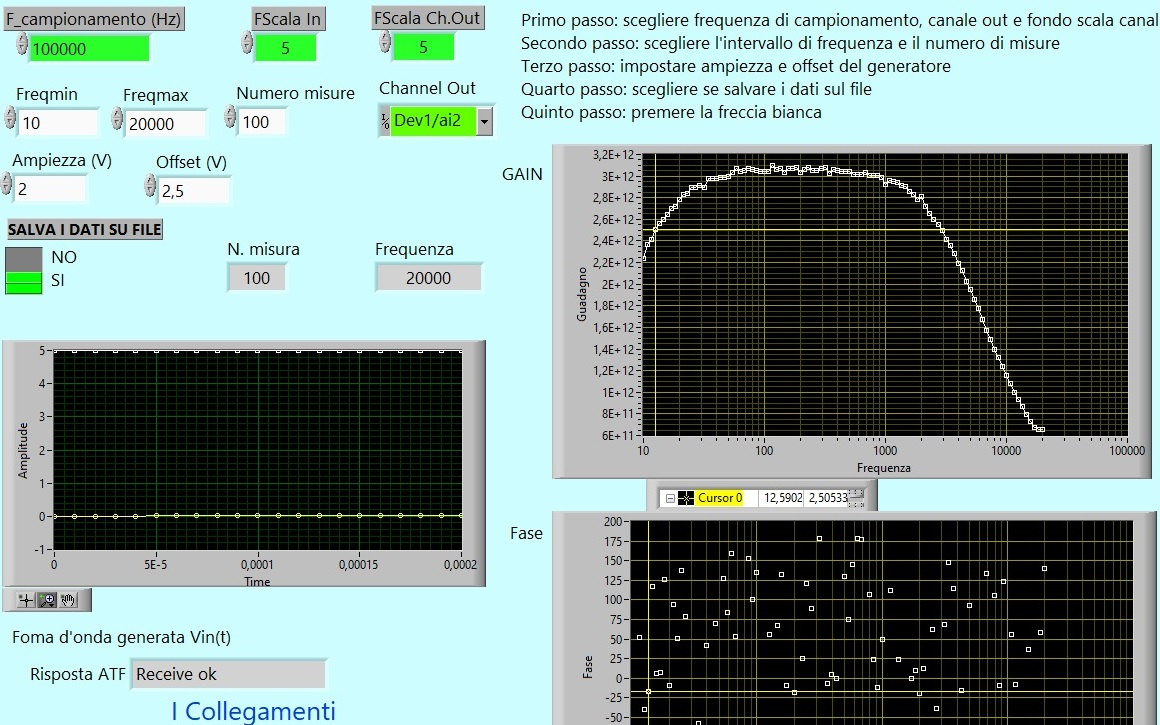
\includegraphics[width=12cm]{settimana_2/immagini/rccr_8.jpg}
    \centering
\end{figure}

All'interno dei grafici, sono presenti le medesime problematiche delle acquisizioni con il circuito CRRC ed offset non nullo. Cercheremo di studiare nel dettaglio tale condizione attraverso il confronto con le successive acquisizioni.

\LogMark{Acquisizione 9}{15.59}
Ritentiamo diminuendo l'offset a 1V ond'evitare di rischiare di mandare il segnale V\textsubscript{in} in saturazione. Il risultato è il medesimo:

\begin{figure}[H]
\caption{}
    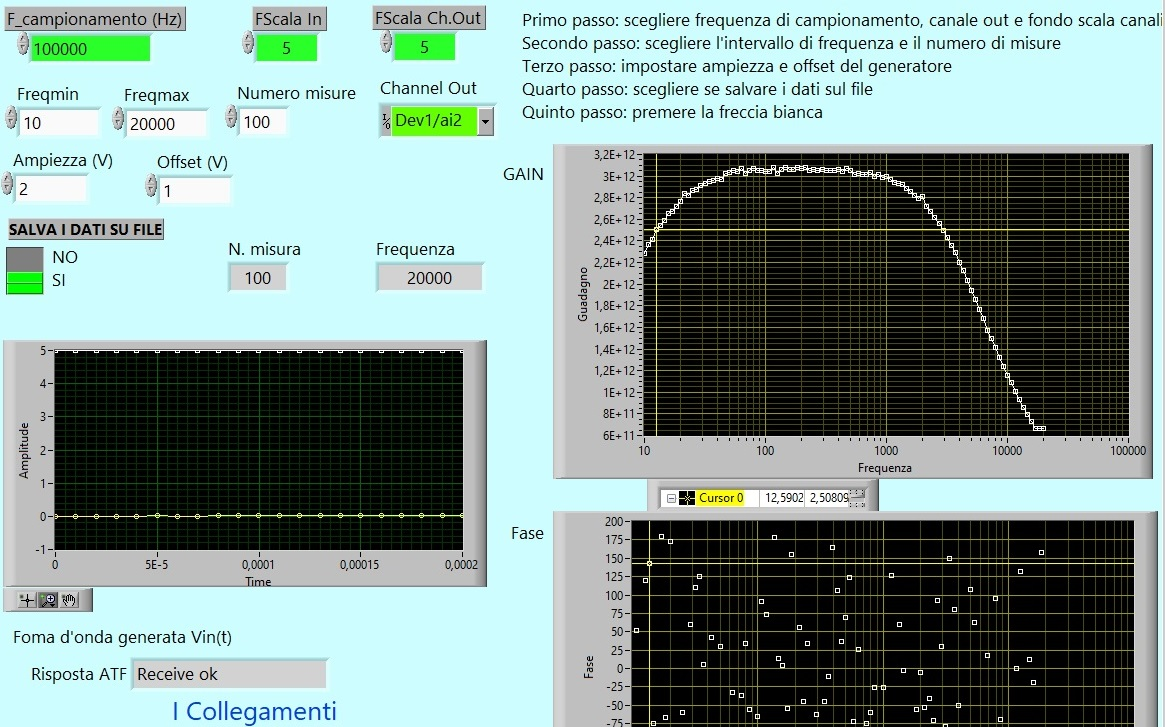
\includegraphics[width=12cm]{settimana_2/immagini/rccr_9.jpg}
    \centering
\end{figure}

\LogMark{Consulto con il professore}{16:20}
Abbiamo fatto varie prove cambiando gli offset, mentre il professore poteva darci delle letture sugli strumenti di laboratorio: scegliendo l'offset di 0.1V, quello effetivamente impostato sul generatore di forme d'onda risultava 1V. Scegliendo l'offset 0.5V (dunque 5V sul generatore) il segnale risultava tagliato. Abbiamo concluso che questo era l'effettivo problema nelle acquisizioni precedenti.

\Importate{
    L'offset viene comunicato al generatore di funzioni con un fattore x10, questo potrebbe spiegare i problemi riscontrati con gli offset
}

Dopo aver parlato col professore, ripetiamo le prove da lui proposte per vedere cosa succede effettivamente mettendo l'offset non nullo. Notiamo che, per un determinato range di valori delle ampiezze in ingresso, la scala di offset risulta in realtà moltiplicata per un fattore 10 rispetto a quanto scritto nella piattaforma. 
Il professore ci ha fatto vedere che all'interno del VI di acquisizione è specificato che l'offset risulta moltiplicato per un fattore, il cui valore dipende dalla scelta effettuata per l'ampiezza di ingresso. Quindi grazie a ciò, è possibile spiegare i risultati ottenuti. 
Di seguito elenchiamo le prove fatte e quanto osservato:
\begin{enumerate}
    \item offset impostato a 0.1V, il valore effettivamente impostato risultava 1V;
    \item offset impostato a 0.5V, il valore effettivamente impostato risultava 5V e il frafico del segnale nel dominio dei dempi di V\textsubscript{in} risultava solo in parte saturato.
\end{enumerate}

Successivamente, al fine di documentare i test appensa eseguiti, li ripetiamo salvando i dati prodotti (acquisizione 10 e 11).

\LogMark{Acquisizione 10}{16:30}
Nella presente acquisizione, impostiamo il valore dell'offset a 0.1 V. dal grafico sottostante, notiamo che l'offset effettivo in realtà è di 1 V (a sostegno di quanto detto nel punto precedente).

\begin{figure}[H]
\caption{}
    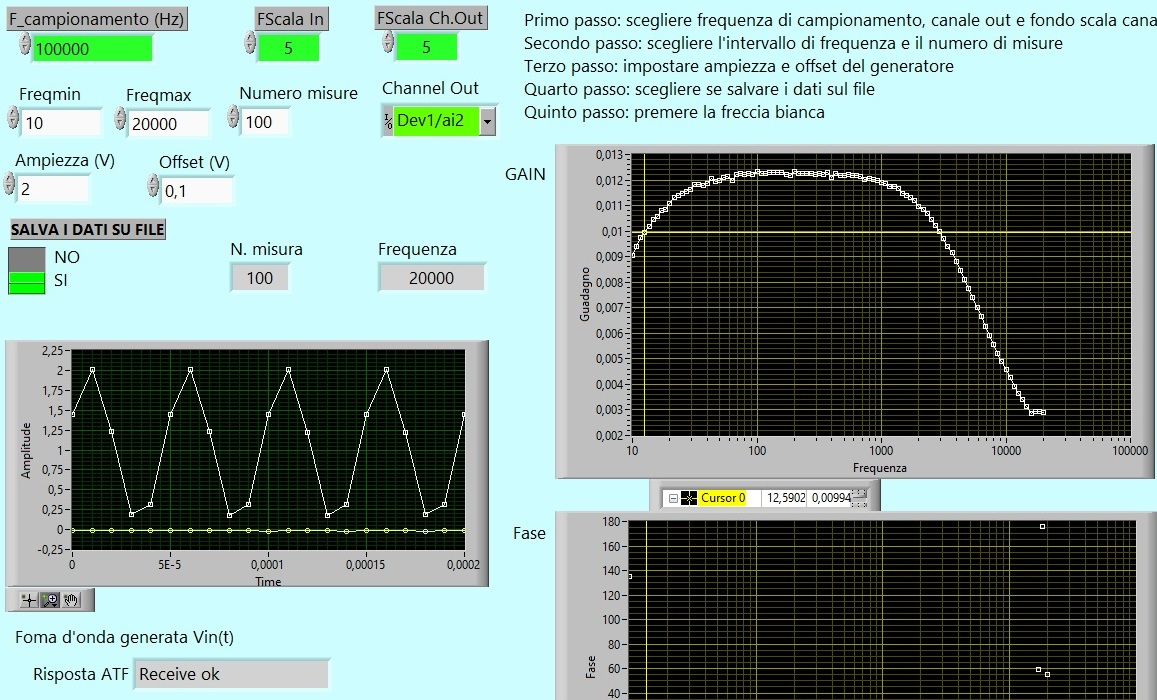
\includegraphics[width=12cm]{settimana_2/immagini/rccr_10.jpg}
    \centering
\end{figure}

\LogMark{Acquisizione 11}{16:31}
Nella presente acquisizione, impostiamo il valore dell'offset a 0.5 V. Dal grafico sottostante, notiamo che l'offset effettivo in realtà è di 5 V. L'onda risulta, infatti, segata a metà, avendo le semionde positive appianate a 5 V (valore di fondo scala).

\begin{figure}[H]
\caption{}
    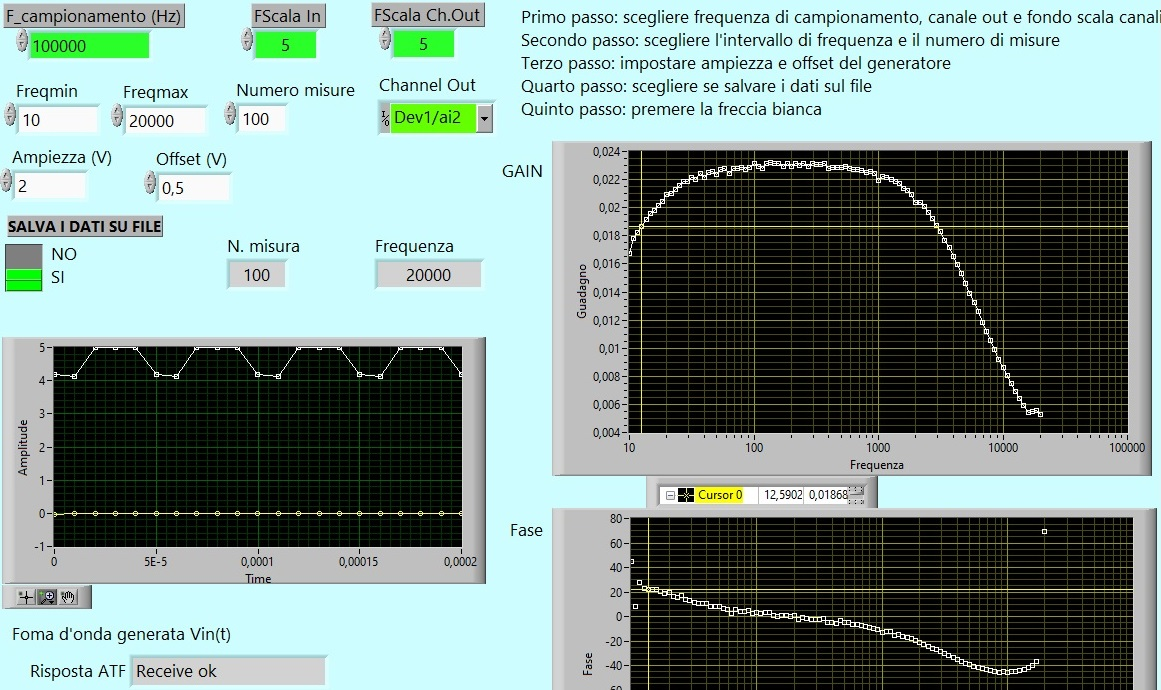
\includegraphics[width=12cm]{settimana_2/immagini/rccr_11.jpg}
    \centering
\end{figure}

\LogMark{Acquisizione 12}{16.33}
Impostiamo i seguenti parametri:
\begin{itemize}
    \item I fondi scala del segnale di ingresso e di uscita rispettivamente a 0.5 V e 0.05 V;
    \item l'ampiezza a 0.1 V
    \item la frequenza minima e massima rispettivamente a 5 Hz e 20 kHz;
    \item il numero di misure a 100
    \item l'offset a zero
\end{itemize} E poniamo l'amiezza in ingresso a 0.1 V
Lo scopo di questa acquisizione, infatti, è analizzare l'acquisizione ad ampiezze molto poco elevate. 

\begin{figure}[H]
\caption{}
    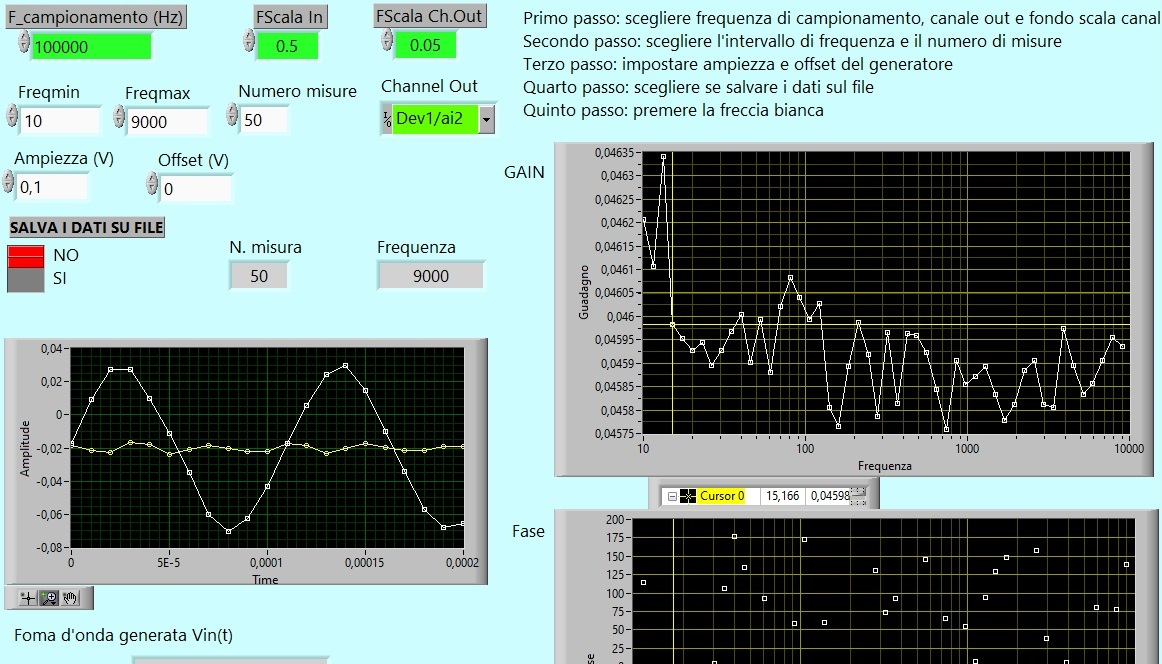
\includegraphics[width=12cm]{settimana_2/immagini/rccr_13.jpg}
    \centering
\end{figure}

Il grafico non risulta affatto in accordo con l'andamento ed i valori quantitativi ideali. Pensiamo che questo sia dovuto ad un fondo scala del secondo canale troppo piccolo.
\Avvertimento{
    Abbiamo osservato successivamente che esso somiglia addirittura ad un segnale di rumore, con sfasamento ed ampiezza soggetta a sole piccole fluttuazioni in ordinata. Infantti guardando il grafico nel dominio del tempo del secondo canale vediamo che i dati sembrano avere natura casuale. La prova fatta successivamente non ha quindi alcun significato.
}

\LogMark{Acquisizione 13}{16.38}
Aumentiamo il fondoscala del segnale in uscita a 0.5 V. I risultati non variano significativamente dai precedenti e per tale motivo non riportiamo i grafici (i dati sono comunque disponibili all'interno della cartella).

\Avvertimento{
    Per le acquisizioni precedenti non abbiamo considerato l'opzione di utilizzare due fondi scala differenti. Ciò avrebbe sicuramnte migliorato l'incertezza sulle stime dei guadagni, visto che quello massimo è di circa 0.015.
}

\NewDay{Altre acquisizioni libere}{02/10/2020}
\LogMark{Ulteriori acquisizioni per il filtro CRRC}{9.36}
All'interno delle acquisizioni del segnale in uscita dal filtro CRRC, realizzate in data 29/09/2020, non è stata analizzata la risposta del circuito a bassa frequenza. In luogo di ciò, ritorniamo alla relativa piattaforma web e lanciamo un'acquisizione che spazi tra 5 Hz e 10 kHz, con frequenza di campionamento di 0.2 MeSa/s e numero di misure pari a 100. Il risultato ottenuto è mostrato in figura:

\begin{figure}[H]
\caption{}
    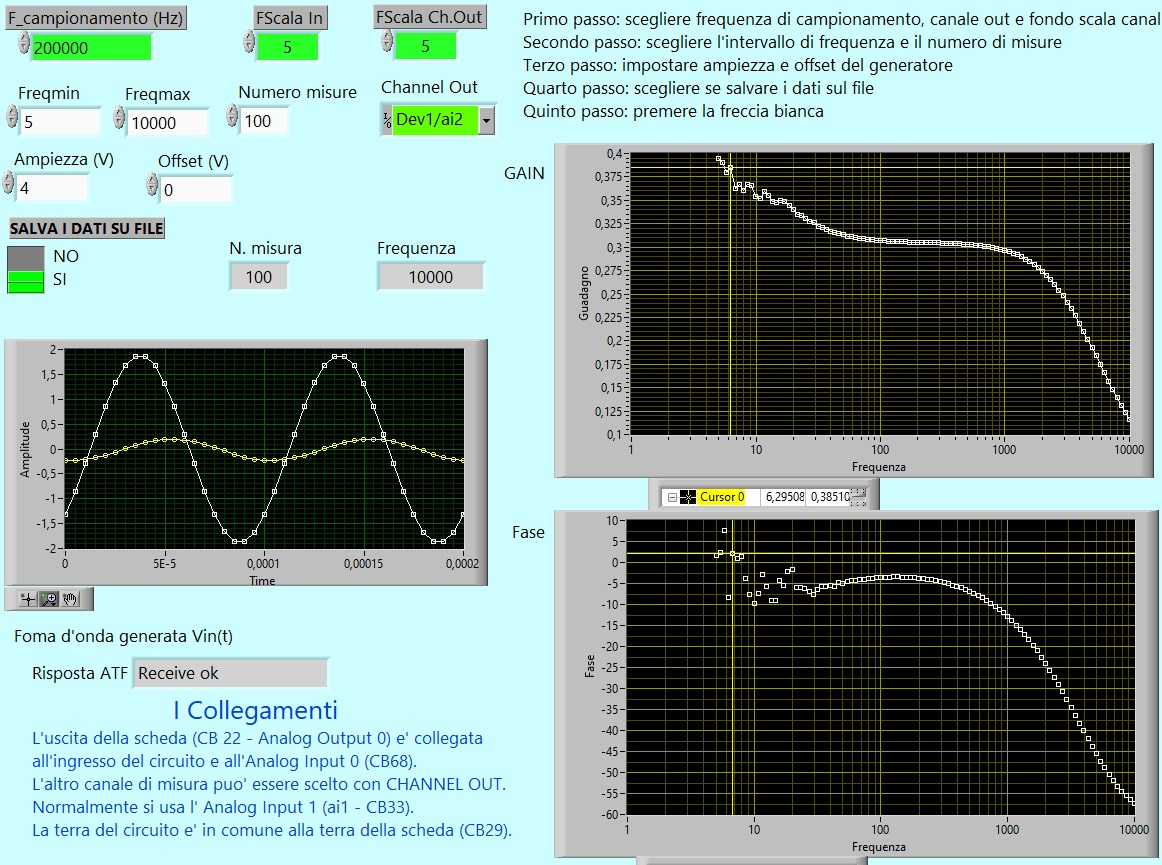
\includegraphics[width=12cm]{settimana_2/immagini/CRRC_1_nuovo.jpg}
    \centering
\end{figure}

Vediamo che a basse frequenze il guadagno tende ad aumentare e l'andamento risulta molto diverso da quello aspettato. Non essendo noto il funzionamento del programma di analisi all'interno del VI atto all'acquisizione dati e la stima dei parametri, consideriamo la possibilità che quest'ultima possa risultare fallacea quando un segnale a bassa frequenza viene campionato con una frequenza di campionamento abbastanza elevata e possibilmente sovrapposto a rumore.

\LogMark{Prova con minore frequenza di campionamento}{9:40}
Per cercare di ottenere delle informazioni significative sul comportamento alle basse frequenze, proviamo a diminuire il sampling rate, impostandolo a 0.1MeSa/s.

\begin{figure}[H]
\caption{}
    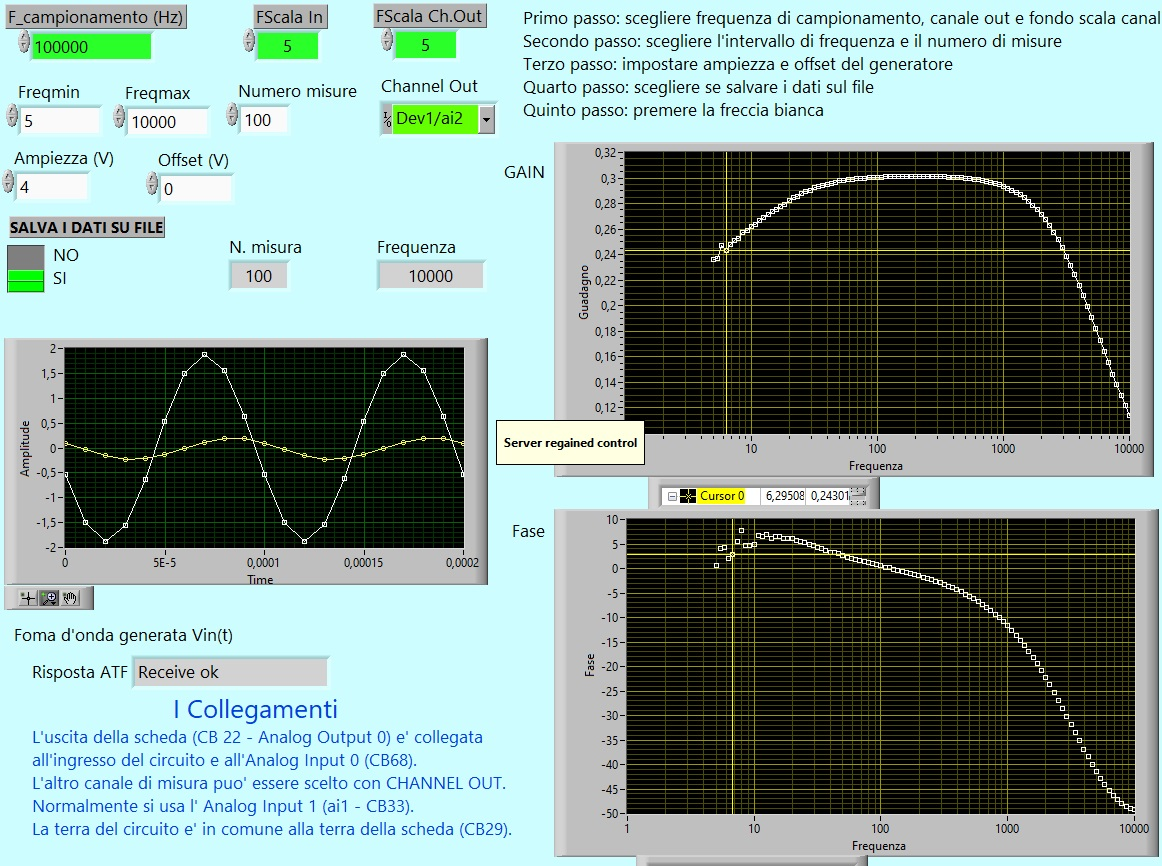
\includegraphics[width=12cm]{settimana_2/immagini/CRRC_2_nuovo.jpg}
    \centering
\end{figure}

In tal caso gli andamenti del guadagno e dello sfasamento sono visivamente più simili a quelli attesi. Concludiamo dunque che la frequenza di campionamento influisce sulla qualità dell'acquisizione a basse frequenze, a sostegno delle argomentazioni fatte nella presa dati precedente.

\Avvertimento{
    Per campionare segnali a bassa frequenza è necessario scegliere un opportuno sampling rate, non troppo alto: per la nostra scheda una regola grezza è 0.1 MeSa/s per segnali ~10Hz.
}

Ora per osservare l'andamento dei dati in un range di frequenze più elevato, poniamo la frequenza massima pari a 20 kHz, lasciando invariati gli altri parametri. Il risultato è mostrato in figura:
\begin{figure}[H]
\caption{}
    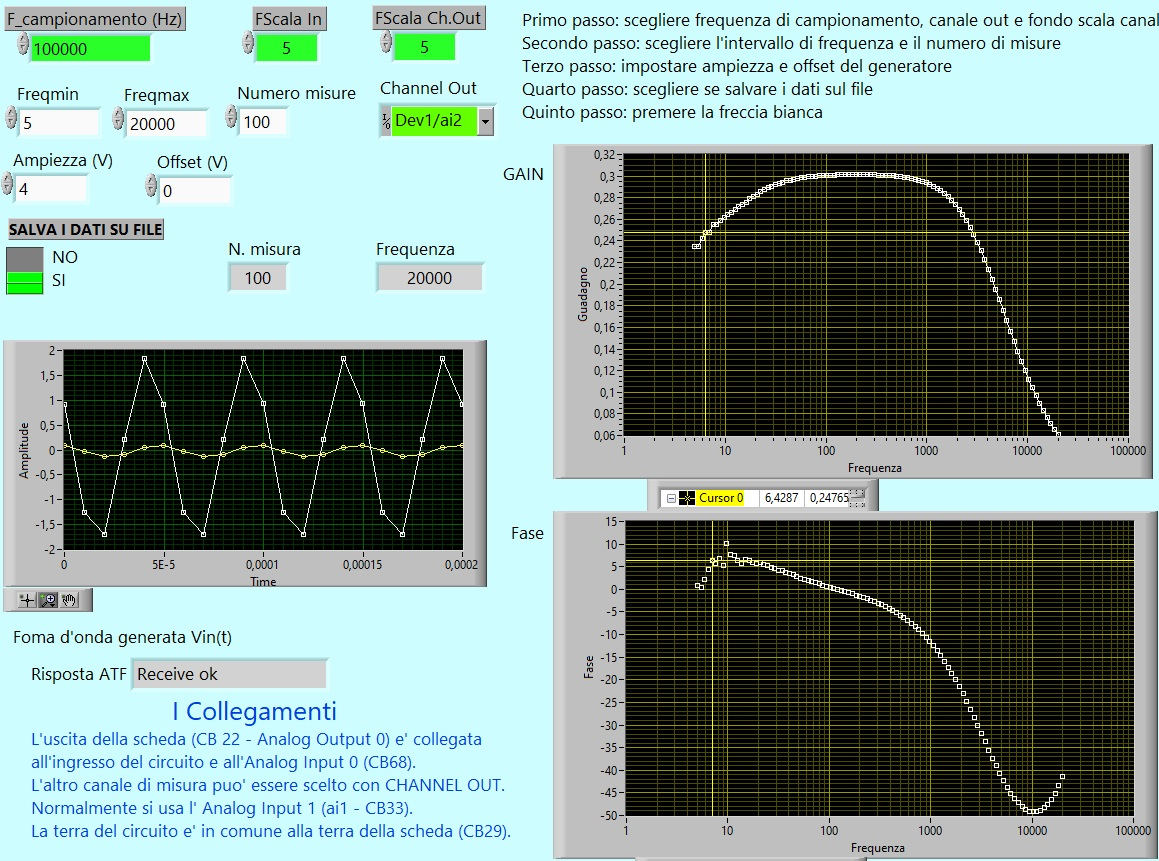
\includegraphics[width=12cm]{settimana_2/immagini/CRRC_3_nuovo.jpg}
    \centering
\end{figure}

\NewDay{Elaborazioni dati ed esercizi}{03/10/2020}

\NewSection{Continuazione scheda prima settimana}

\LogMark{Hw. 2}{11:06}
Riprendiamo il circuito del ponte di Wheatstone realizzato in data 26/09/2020. Attraverso il comando
\begin{equation}
    \text{Analysis} \Rightarrow \text{DC Analysis} \Rightarrow \text{Table of Results}
\end{equation}
All'interno della tabella dei risultati sono presenti i valori delle tensioni e delle intensità di corrente nei vari rami del circuito. La corrente che scorre attraverso l'amperometro (collegato come in figura \ref{fig::ponte}) risulta essere: $I_{amp} = 294.12 \: \mu A$.


\LogMark{Hw. 3}{11:20}
Modifichiamo il valore della resistenza $R_2$, ponendola pari a $R_X$. Dopodiché apriamo la tabella dei risultati e osserviamo che la corrente che scorre nell'amperometro risulta essere nulla.

\Nota{
    Hw. 4 è stato fatto a lezione.
}

\LogMark{Hw. 5}{11:28}

All'interno dell'ambiente simulzione TINA abbiamo adottato un generatore di tensione ideale. Dunque dall'analisi del circuito ci aspetteremo di avere:
\begin{equation}
    I_{amp} = V_0\frac{R_2 R_3 - R_1 R_X}{R_1 R_x R_3 + R_2 R_x R_3 + R1 R_2 R_x + R1 R_2 R_3}
    \label{eq::ponte}
\end{equation}
Inserendo i valori nominali dell'homework 2 e la precedente espressione all'interno dello shell di Matlab, otteniamo il seguente valore per la corrente che scorre nell'amperometro: $I_{amp} = 294.1176 \: \mu A $. Il risultato è in accordo con quanto letto all'interno della tabella dei risultati in TINA.
Per vedere ulteriormente che la formula è corretta, impostiamo il valore della resistenza $R_2$ a 10 $k\Omega$. Il risultato letto all'interno dei tabella dei risultati di TINA e quello calcolato con Matlab sono rispettivamente: $479.45 \: \mu A$ e $479.4521 \: \mu A$, che risultano in accordo, come ci saremo aspettavamo.

\LogMark{Hw. 6}{11:40}
Ritorniamo al circuito del ponte realizzato in TINA ed azioniamo il comando:
\begin{equation}
    \text{Analysis} \Rightarrow \text{DC Analysis} \Rightarrow \text{DC Transfer Characteristic}
\end{equation}
Scegliamo la resistenza $R_2$ e la facciamo variare da 400 $\Omega$ a 4 $k\Omega$. Premendo "ok", otteniamo il grafico della corrente misurata dall'amperometro $I_{amp}$ in funzione del valore della resistenza $R_2$. Con un cursore verifichiamo che lo zero della funzione corrisponde effettivamente a $R_2 = 3 \: k\Omega$. Inseriamo una griglia, modifichiamo le scale ed i nomi degli assi affinchè possiamo avere una visualizzazione ottimale. Il grafico ottenuto è riportato di seguito:

\begin{figure}[H]
\caption{}
    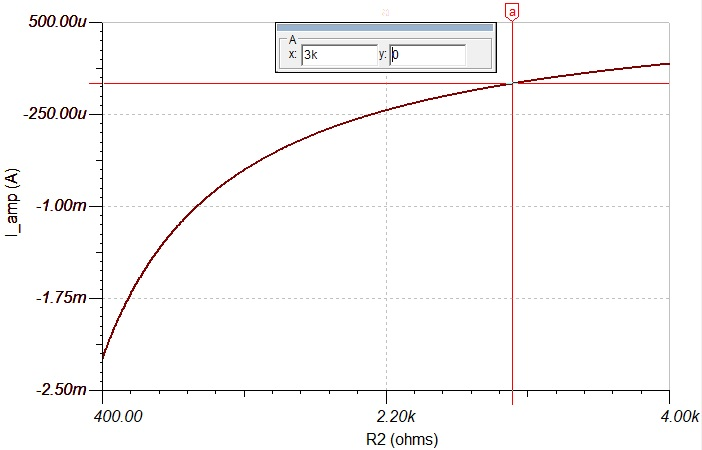
\includegraphics[width=7cm]{settimana_2/immagini/diagramma_r2.jpg}
    \centering
\end{figure}

\LogMark{Hw. 7}{12:04}
Attraverso l'ambiente Matlab, eseguiamo le seguenti operazioni attraverso la shell:

\begin{verbatim}
    R1 = 1e3;
    R3 = 1e3;
    Rx = 3e3;
    syms R2;
    I =         V0 * (R2 * R3 - R1 * Rx) / ...
        (R1*Rx*R3 + R2*Rx*R3 + R1*R2*Rx + R1*R2*R3);
    fplot(I, [400, 4e3])
\end{verbatim}

Il risultato dell'operazione è un grafico in cui è riportata la funzione \ref{eq::ponte}, fissando le variabili $R_1$, $R_3$ e $R_x$ come specificato nella consegna dell'homework 2 e usando quale variabile uindipendente $R_2$. Quest'ultima viene fatta variare all'interno del range $[400 \: \Omega, \: 4 \: k\Omega]$. Inseriamo una griglia, modifichiamo le scale ed i nomi degli assi ai fini di una visualizzazione ottimale. Di seguito riportiamo il grafico ottenuto:
\begin{figure}[H]
\caption{}
    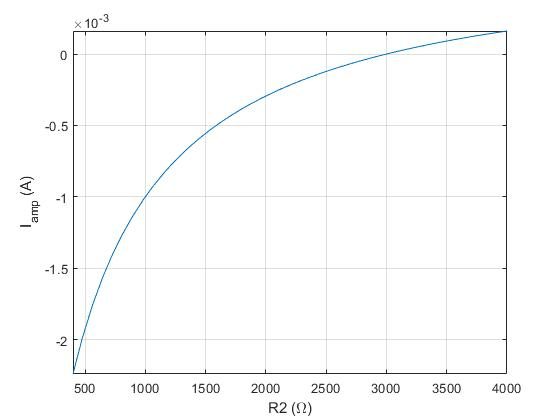
\includegraphics[width=7cm]{settimana_2/immagini/diagramma_r2_matlab.jpg}
    \centering
\end{figure}
Il grafico risulta corrispondere con quello realizzato attraverso la simulazione in TINA.

\LogMark{Hw. 8}{12:25}
All'interno del circuito \ref{fig::ponte}, sostiuiamo l'amperometro con una resistenza $R_5$ di 1 $\Omega$ (bassa rispetto alle resistenze presenti negli altri rami). Adottando il comando Table of DC Result, possiamo vedere le correnti e le tensioni ai capi dei vari componenti. Osserviamo che entro $R_5$ scorre una corrente pari a $I_{5} = \: 293.91 \mu A$.
Il valore risulta simile a quello ottenuto con l'amperometro. Proviamo, comunque, a diminuire la resistenza a $R_{5} = 1 \: m\Omega$ per vedere se il risultato risulta più concorde alle aspettative rispetto al precedente. All'interno della tabella dei risultati DC, leggiamo che la corrente che scorre in $R_5$ è pari a $I_{5} = \: 294.12 \mu A$, che risulta effettivamente in accordo con quanto letto se invece di $R_5$ ci fosse un amperometro.
Proviamo ora a vedere come varia la corrente sul ramo di $R_5$ aumentando l'omonima resistenza. I risultati sono riportati in tabella:
\begin{center}
\begin{tabular}{|c|c|c|c|c|c|c|c|c|}
\hline
$\textbf{R}_{\textbf{5}}$         &$10 \: m\Omega$        &$100 \: m\Omega$         &$10 \: \Omega$         &$100 \: \Omega$         &$1 \: k\Omega$         &$10 \: k\Omega$         &$100 \: k\Omega$         &$1 \: Me\Omega$     \\
\hline
$\textbf{I}_{\textbf{5}}$ [$\mu A$]         &$294.12$        &$294.1$         &$292.06$         &$274.73$         &$172.41$         &$36.5$         &$4.11$         &$0.41608$    \\
\hline
\end{tabular}
\end{center}
Osserviamo dunque che la correte tende ad anullarsi all'aumentare della resistenza $R_5$. Ciò risulta ragionevole in quanto più un carico è resistivo, maggiore è l'inerzia che oppone al passaggio di corrente.
Ai fini di analizzare in modo più preciso l'andameno della corrente che scorre in $R_5$ in funzione dell'omonima resistenza, mettiamo un amperometro in serie ad $R_5$. Abbiamo così realizzato un partitore di tensione, in cui la corrente che scorre dunque è uguale per ambedue i componenti. L'amperometro, come è noto, può essere approssimato ad una piccola resistenza r'. Quindi potremo modellare la relazione che intercorre fra $I_{amp}$ e $R_5$ come segue:
\begin{equation}
    I_{amp} = \Delta V (R_5 + r') = r \Delta V
\end{equation}
ove $\Delta V$ è la tensione ai capi del partitore ed r è la resistenza equivalente del ramo.
La curva in questione non è una retta. Infatti i parametri $\Delta V$ e $I_{amp}$ possono variare anche per via dei rapporti della resistenza del ramo di $R_5$ con quelle degli altri rami del circuito. Più precisamente dovrà valere la legge:
\begin{equation*}
    I_r = V_{0}\,\frac{R_{2}R_{3}-R_{1}R_{x}}{R_{1}R_{2}\,R_{3}+R_{1}R_{2}R_{x}+R_{1}R_{3}R_{x}+R_{2}R_{3}R_{x}+R_{1}R_{3}r+R_{2}R_{3}r+R_{1}R_{x}r+R_{2}R_{x}r}
\end{equation*}
ove $I_5$ è stato rinominaro $I_r$ per porre in luce che questa è la corrente che scorre sulla resistenza equivalente.
Quindi l'andamento sarà più simile ad un ramo d'iperbole del tipo:
\begin{equation}
    I_r = {A\over {B + C \cdot r}}
\end{equation}
con A, B e C costanti dipendenti da caratteristiche costruttive del circuito.
Quello che osserviamo usando il comando AC Transfer Characteristic è il grafico seguente:
\begin{figure}[H]
\caption{}
    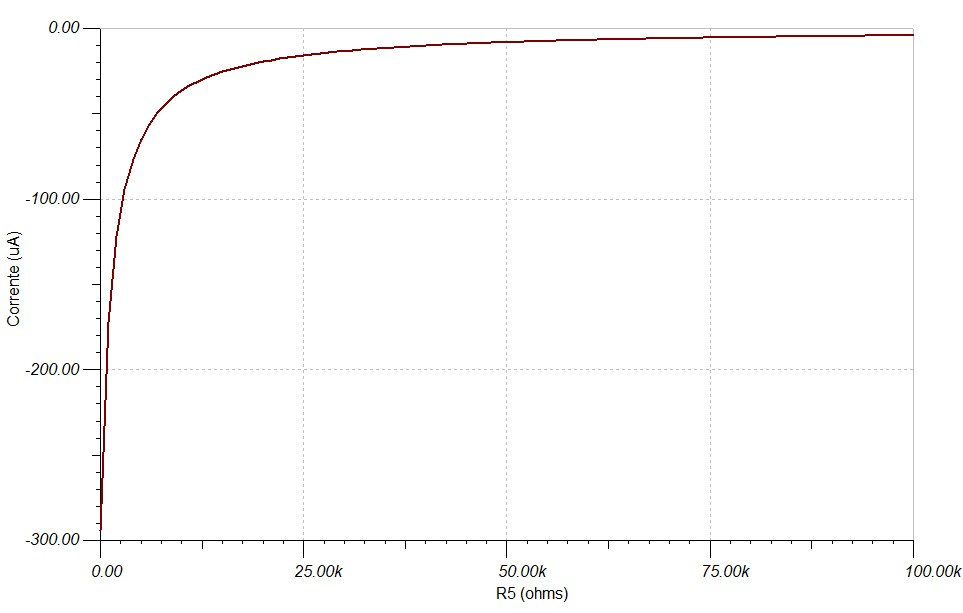
\includegraphics[width=10cm]{settimana_2/immagini/IvsR5.jpg}
    \centering
\end{figure}
E' stato spaziato un range di valori di resistenza per $R_5$ pari a $[0, 100]\:  k\Omega$. Osserviamo che, a parte il segno negativo dovuto al verso in cui è stato inserito l'amperometro nel ramo, la corrente risulta tendere a 0 ed a diminuire in modulo per valori crescenti di $R_5$.Ai fini di osservare più accuratamente cosa succede per bassi valori di resistenze realizziamo un secondo grafico, che riportiamo di seguito:
\begin{figure}[H]
\caption{}
    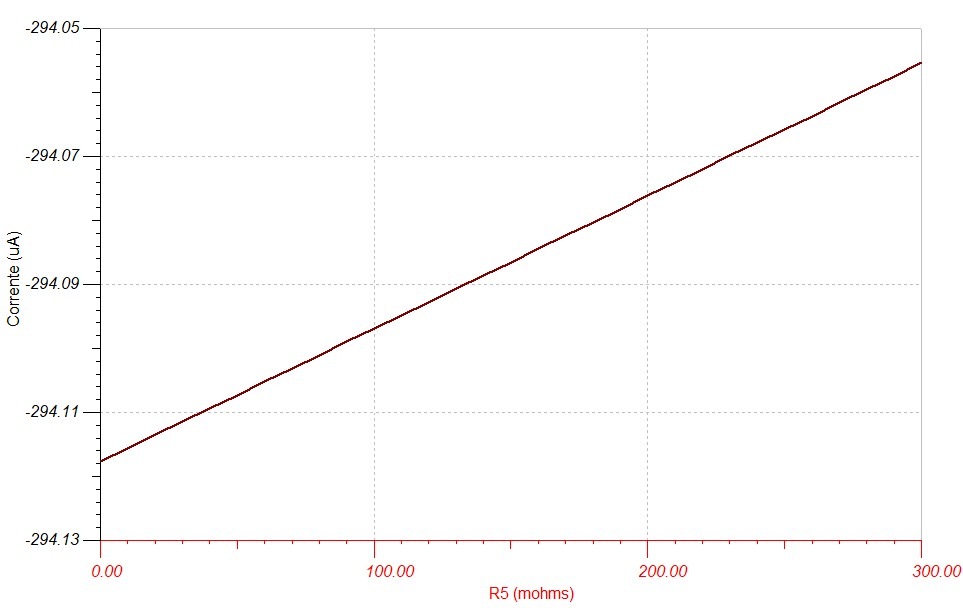
\includegraphics[width=10cm]{settimana_2/immagini/IvspiccoleR5.jpg}
    \centering
\end{figure}
la quale è come da aspettarsi una retta del tipo:
\begin{equation}
    I_r \approx {A\over{B}} - r {{A C}\over{B^2}} = ({A\over{B}} - r' {{A C}\over{B^2}}) - R_5 {{A C}\over{B^2}}  
\end{equation}
ove A, B e C sono i parametri introdotti precedentemente, i quali dipendono dalle sole impedenze dei altri rami del circuito e dalla tensione ai capi del ponte, che sono parametri che rimangono costanti all'interno della presente simulazione.
Ora eliminiamo nuovamente l'amperometro dal ramo. Vogliamo osservare per quale valore di $R_5$ la corrente $I_5$ risulta diminuita di circa il $10 \%$ (quindi $I_5 \approx 264.71 \: \mu A$) del valore originariamente misurato col solo amperometro. Dalla tabella, ove avevamo riportato i valori della corrente $I_5$ e della resistenza $R_5$, osserviamo che la resistenza cercata si ha entro la decade $[100 \: \Omega, \: 1 \: k\Omega]$.
Faccio delle prove, nell'ordine che va da destra a sinistra nella seguente tabella, per trovare approssimativamente il valore giusto:
\begin{center}
\begin{tabular}{|c|c|c|c|c|c|c|c|c|}
\hline
$\textbf{R}_{\textbf{5}}$        &$500 \: \Omega$        &$250 \: \Omega$        &$200 \: \Omega$        &$150 \: \Omega$        &$175 \: \Omega$        &$160 \: \Omega$        &$158 \: \Omega$        &$157 \: \Omega$        \\
\hline
$\textbf{I}_{\textbf{5}}$ [$\mu A$]         &$217.39 \: \mu A$        &$250.00 \: \mu A$        &$253.73 \: \mu A$        &$265.96 \: \mu A$        &$261.78 \: \mu A$        &$264.27 \: \mu A$        &$264.61 \: \mu A$        &$264.77 \: \mu A$        \\
\hline
\end{tabular}
\end{center}
Quindi posso affermare che la perturbazione risulta superiore del $10\%$ per valori $R_5 \approx 158 \: \Omega$.
Osserviamo che con le accortezze prese in questa analisi, si è tenuta conto della resistenza finita dell'amperometro e che l'unica fonte incertezza è puramente computazionale.

\LogMark{Hw. 9}{12:40}
Con gli strumenti simbolici di Matlab è stata modellata la corrente sull'amperometro di resistenza $r$:
\begin{equation*}
    I_r = V_{0}\,\frac{R_{2}R_{3}-R_{1}R_{x}}{R_{1}R_{2}\,R_{3}+R_{1}R_{2}R_{x}+R_{1}R_{3}R_{x}+R_{2}R_{3}R_{x}+R_{1}R_{3}r+R_{2}R_{3}r+R_{1}R_{x}r+R_{2}R_{x}r}
\end{equation*}

Facendo il limite per $r \rightarrow 0$ con il comando \verb|limit(I_r, r, 0)| si trova la legge atttesa:
\begin{equation*}
    V_{0}\,\frac{R_{2}\,R_{3}-R_{1}\,R_{x}}{R_{1}\,R_{2}\,R_{3}+R_{1}\,R_{2}\,R_{x}+R_{1}\,R_{3}\,R_{x}+R_{2}\,R_{3}\,R_{x}}
\end{equation*}.

Come verifica grafica, proviamo a disegnare in scala logaritmica $I_r(r)$ per i parametri scelti:
\begin{figure}[H]
\caption{}
    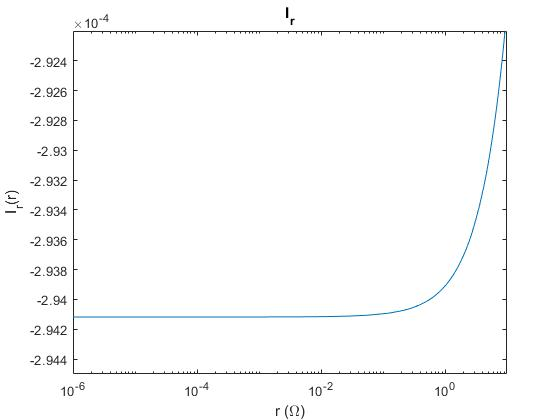
\includegraphics[width=7cm]{settimana_2/immagini/I_r.jpg}
    \centering
\end{figure}

Aumentando la resistenza $r$, la corrente sull'amperometro diminuisce, vogliamo racavare quando la differenza con il valore per $r = 0$ supera il 10\%. Chiamando $I_0$ il valore della corrente per $r = 0$ si vuole risolvere:
\begin{equation*}
    I_r = I_0 \cdot 0.9
\end{equation*}.

Per farlo utilizziamo il comando \verb|solve(f_Ir - I_1, r)| ottenendo un valore di $157 \Omega$, simile a quello trovato manualmente con TINA.


\NewDay{Completamento della seconda scheda}{04/10/2020}

\NewSection{Analisi formale circuito CRRC}

\LogMark{Funzione di trasferimento, guadagno e sfasamento - Es. 5}{16.00}

Attraverso gli strumenti simbolici di Matlab abbiamo modellizzato il circuito CRRC con il metodo simbolico, per trovarne la funzione di trasferimento.

Creiamo dapprima la funzione per calcolare l'impedenza di un condensatore:
\begin{lstlisting}[frame=single]
function [Z] = impedenza_condensatore(c, omega)
    Z = 1 / (j  * omega * c);
end
\end{lstlisting}

e quello per calcocare la tensione e l'impedenza di thevenin per un circuito come in figura \ref{fig:partitore} (partitore di tensione con impedenze R1 e R2):
\begin{figure}[H]
  \caption{}
  \centering
    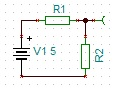
\includegraphics[width=0.3\textwidth]{settimana_2/immagini/partitore.jpg}
    \label{fig:partitore}
\end{figure}
\begin{lstlisting}[frame=single]
function [ratio_Vth_Vin, Rth] = calcola_thevenin(r1, r2)
    ratio_Vth_Vin = 1 / (r1/r2 + 1);
    Rth = 1 / (1/r1 + 1/r2);
end
\end{lstlisting}

Considerando la parte del circuito a sinistra (generatore, C1 e R1) e imponendo unitaria l'ampiezza della tensione del generatore, la modellizziamo come un generatore di thevenin:
\begin{lstlisting}[frame=single]
[Vth, Rth] = calcola_thevenin(impedenza_condensatore(C1, omega), R1)
\end{lstlisting}

Consideriamo ora la serie R2-C2 e calcoliamo la corrente su di questa:
\begin{lstlisting}[frame=single]
Z2 = impedenza_condensatore(C2, omega) + R2
I2 = Vth / (Rth + Z2)
\end{lstlisting}

La tensione V\textsubscript{out} si calcola come:
\begin{lstlisting}[frame=single]
Vout = I2 * impedenza_condensatore(C2, omega)
\end{lstlisting}

Possiamo infine definire la funzione di trasferimento del circuito $H_{CRRC}$, il guadagno $A$ e lo sfasamento $\theta$ come:
\begin{lstlisting}[frame=single]
H_CRRC = Vout
A = sqrt((conj(H_CRRC) * H_CRRC))
tanTheta = imag(H_CRRC) / real(H_CRRC)
\end{lstlisting}

Dopo le opportune semplificazioni si ha:
\begin{equation}
\begin{array}{l}
    H_{CRRC} = \frac{C_1 \,f\,f_b \,\mathrm{i}}{C_1 \,f_a \,f_b -C_1 \,f^2 +C_1 \,f\,f_a \,\mathrm{i}+C_1 \,f\,f_b \,\mathrm{i}+C_2 \,f\,f_b \,\mathrm{i}}\\\\
    \text{con } f_a = \frac{1}{C_1 R_1} \text{ e } f_b = \frac{1}{C_2 R_2}
\end{array}
\end{equation}
 e se $f \neq 0$:
\begin{equation}
    H_{CRRC} = \frac{1}{i(\frac{f_a}{f} - \frac{f}{f_b}) - (\frac{fa}{fb} + 1 + \frac{C_2}{C_1})}
\end{equation}

Inoltre:
\begin{equation}
    A_{CRRC} = {1\over{\sqrt{({f_a\over{f_b}} + 1 + {C_2\over{C_1}})^2 + ({{f^2 - f_a f_b}\over{f f_b}})^2}}}
\end{equation}
\begin{equation}
    {\theta}_{CRRC} = \arctan{\frac{C_1 \,{\left(f_a \,f_b -f^2 \right)}}{f\,{\left(C_1 \,f_a +C_1 \,f_b +C_2 \,f_b \right)}}}
\end{equation}
Di seguito riportiamo i grafici in scala logaritmica del guadagno e dello sfasamento per un range di frequenze pari a $[1 \: Hz, \: 10 \: kHz]$:

\begin{figure}[H]
\caption{}
	\centering
	\begin{subfigure}
	\centering
		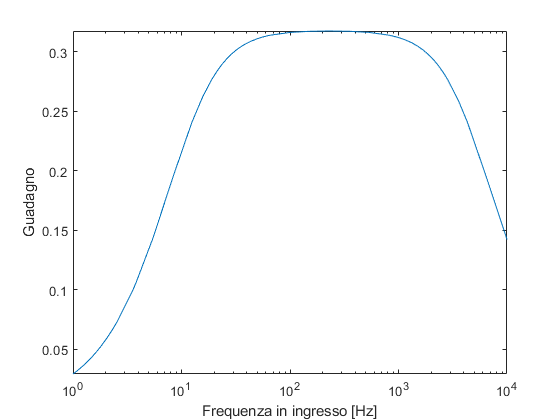
\includegraphics[width=7cm]{settimana_2/immagini/CRRCguadagno.png}
	\end{subfigure}
	\begin{subfigure}
	\centering
		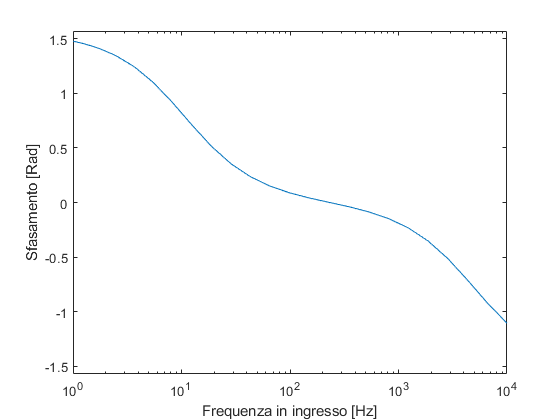
\includegraphics[width=7cm]{settimana_2/immagini/CRRCsfasamento.png}
	\end{subfigure}
\end{figure}
%[width=7cm]

\LogMark{frequenza di massimo trasferimento CRRC Es. 6}{18.00}
Eseguiamo la derivata del guadagno in funzione della frequenza f secondo il comando:
\begin{lstlisting}[frame=single]
A_1 = diff(A, f);
\end{lstlisting}
Dopodichè risolviamo l'equazione:
\begin{equation}
    {{\partial A} \over{\partial f}} = 0
\end{equation}
per trovare un punto stazionario, il quale corrisponderà al massimo della funzione guadagno al variare della frequenza.
Per farlo adottiamo i seguenti comandi:
\begin{lstlisting}[frame=single]
f_max = solve(A_1, f)
A_max = subs(A, f, f_max)
\end{lstlisting}
La frequenza per cui si ha il guadagno massimo risulta essere (dopo le dovute semplificazioni):
\begin{equation}
    f_{max} = \sqrt{f_a f_b}
\end{equation}
per la quale il guadagno risulta essere:
\begin{equation}
    max(A) = {1\over{ {f_a\over{f_b}} + 1 + {C_2\over{C_1}}}}
\end{equation}
Per analizzare la dipendenza di $f_{max}$ dal valore di $R_2$, riscriviamo l'espressione precedentemente trovata come:
\begin{equation}
    f_{max} = {1 \over{2 \pi \sqrt{R_1 C_1 R_2 C_2}}} \propto R_2^{-{1\over{2}}}
\end{equation}
ove le sostituzioni sono ovvie. Quindi la frequenza $f_{max}$ varia proporzionalmente al r della radice della resistenza $R_2$. Conseguentemente, all'aumentare di $R_2$ la frequenza per cui si ha il massimo del guadagno A diminuisce.

\LogMark{Usare il circuito CRRC per mandare segnale ad un utilizzatore esterno - Es. 7}{19.38}
Vogliamo analizzare cosa succede se il circuito il segnale in uscita dal circuito CRRC viene mandato su un carico con bassa impedenza di ingresso.  

Abbiamo visto che il circuito in questione si può modellizzare come un attenuatore lineare con funzione di trasferimetno $H_{CRRC}$. Possiamo applicare il metodo di thevenin, ottenendo che $V_{th} = H_{CRRC}(\omega)V_{\omega \, in}$, mentre per l'impedenza $Z_{th}$ adottiamo il comando:
\begin{lstlisting}[frame=single]
[~, Rth] = calcola_thevenin(impedenza_condensatore(C2, omega), R2 + Rth1
\end{lstlisting}
dove Rth1 è l'impedenza del primo attenuatore calcolata precedentemente. Otteniamo:
\begin{equation}
    Z_{th_{CRRC}} = -\frac{R_2 \,f_b \,{\left(-R_2 \,f+R_1 \,f_a \,\mathrm{i}+R_2 \,f_a \,\mathrm{i}\right)}}{R_2 \,f^2 \,\mathrm{i}+R_1 \,f\,f_a +R_2 \,f\,f_a +R_2 \,f\,f_b -R_2 \,f_a \,f_b \,\mathrm{i}}
\end{equation}

Se guardiamo l'andamento in funzione della frequenza osserviamo come l'impedenza diminuisce alle alte frequenze (perchè diminuiscono quelle dei condensatori), mentre tende a $R_1 + R_2$ quando la frequenza tende a zero (l'impedenza dei condensatori va a infinito):
\begin{figure}[H]
\caption{}
    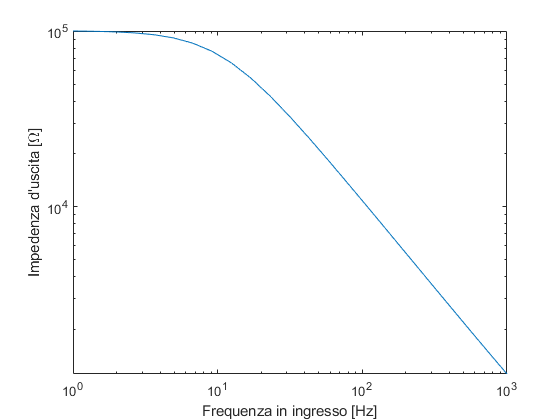
\includegraphics[width=7cm]{settimana_2/immagini/CRRCRth.png}
    \centering
\end{figure}

Se all'uscita del circuido si connette un dispositivo con una bassa impedenza in ingresso, bisognerà allora considerare anche questa nel calcolo della tensione in uscita. In generale avremo una diversa curva di guadagno e sfasamento, le caratteristiche di questa possono dipendere dal tipo di carico connesso (cioè se l'impedenza è reale o complessa).

\NewSection{Analisi formale circuito RCCR}
Come nel caso precedente, utilizziamo gli strumenti simbolici di matlab per modellizzare il circuito. Applichiamo il metodo gei generatori di Thevenin per calcolare la funzione di trasferiemnto. Troviamo:
\begin{equation}
    H_{RCCR} = -\frac{C_2 \,f\,f_b \,{\left(f-f_b \,\mathrm{i}\right)}}{{\left(f_b +f\,\mathrm{i}\right)}\,{\left(C_2 \,f_a \,f_b -C_2 \,f^2 +C_1 \,f\,f_a \,\mathrm{i}+C_2 \,f\,f_a \,\mathrm{i}+C_2 \,f\,f_b \,\mathrm{i}\right)}}
\end{equation}

Da cui:
\begin{equation}
    A_{RCCR} = \frac{C_2 ff_b }{\sqrt{{C_1 }^2 f^2 {f_a }^2 +2C_1 C_2 f^2 {f_a }^2 +2C_1 C_2 f^2 f_a f_b +{C_2 }^2 f^4 +{C_2 }^2 f^2 {f_a }^2 +{C_2 }^2 f^2 {f_b }^2 +{C_2 }^2 {f_a }^2 {f_b }^2 }}
\end{equation}
che si può scrivere:
\begin{equation}
    A_{RCCR} = \frac{1}{\sqrt{ (\frac{f_a}{f_b} (\frac{C_1}{C_2} + 1))^2 + \frac{f^2}{f_b^2} + \frac{f_a^2}{f^2}}}
\end{equation}
e
\begin{equation}
    \theta = \arctan{\frac{C_2 \,{\left(f_a \,f_b -f^2 \right)}}{f\,{\left(C_1 \,f_a +C_2 \,f_a +C_2 \,f_b \right)}}}
\end{equation}

Da queste ricaviamo:
\begin{equation}
    f_{max} = \sqrt{f_a f_b}
\end{equation}
\begin{equation}
    A_{max} = \frac{1}{\sqrt{\frac{f_a}{f_b}(\frac{f_a}{f_b}(\frac{C_1}{C_2} + 1)^2 + 2)}}
\end{equation}

I grafici del guadagno e dello sfasamento risultano:
\begin{figure}[H]
\caption{}
	\centering
	\begin{subfigure}
	\centering
		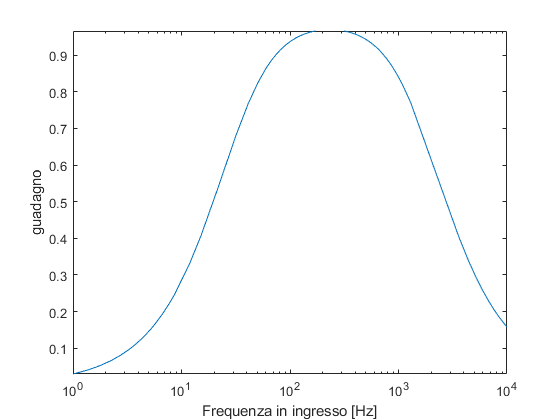
\includegraphics[width=7cm]{settimana_2/immagini/RCCRguadagno.png}
	\end{subfigure}
	\begin{subfigure}
	\centering
		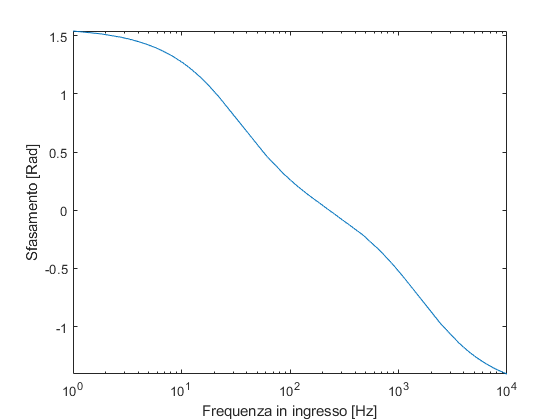
\includegraphics[width=7cm]{settimana_2/immagini/RCCRsfasamento.png}
	\end{subfigure}
\end{figure}

E l'impedenza equivalente di Thevenin:
\begin{equation}
    Z_{th_{RCCR}} = \frac{R_1 \,{\left(R_1 \,f\,f_a +R_2 \,f\,f_b -R_1 \,f_a \,f_b \,\mathrm{i}\right)}}{R_1 \,f^2 \,\mathrm{i}+R_1 \,f\,f_a +R_1 \,f\,f_b +R_2 \,f\,f_b -R_1 \,f_a \,f_b \,\mathrm{i}}
\end{equation}
\begin{figure}[H]
\caption{}
    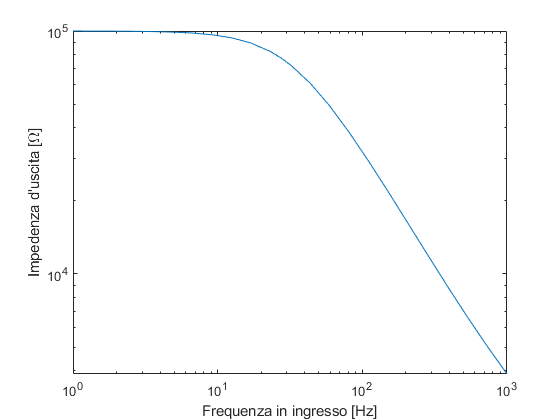
\includegraphics[width=7cm]{settimana_2/immagini/RCCRRth.png}
    \centering
\end{figure}

\NewDay{Analisi dati}{05/10/2020}

\NewSection{Analisi degli sfasamenti per il corto circuito}
Vogliamo indagare sugli sfasamenti osservati nelle acquisizioni con il corto circuito. Osserviamo che questi sembrano suggerire un andamento lineare. Supponendo infatti che la scheda acquisisca sui due canali con uno sfasamento di $\Delta t / 2$, dove $\Delta t = 1/{SR}$ (SR = sampling rate), si ha:
\begin{equation}
     \Delta \phi = {{\pi  f}\over{SR}}
 \end{equation}

Per testare tale ipotesi, analizziamo i dati relativi agli sfasamenti del corto circuito. In particolare utilizziamo i dati dell'acquisizione 2 e 5, facendo un fit ai minimi degli scarti quadrati con una legge di proporzione lineare. Troviamo i coefficienti angolari $m2 = (3.1394 \pm 0.0019) \cdot 10^{-5} \: rad \cdot s$ con $ f_{camp} = 100kHz$ e $m5 = (1.56965 \pm 0.00029) \cdot 10^{-5} \: rad \cdot s$ con $f_{camp} = 200kHz$.

\Nota{
    Si nota un aumento dell'incertezza per valori alti delle frequenze.
}
 %nome immagine = "sfasamentocorrettocorto2.jpg"
  %nome immagine = "sfasamentocorrettocorto5.jpg" (acquis5 f = 200kHz)
% Prima con acquis2 e acquis5.
Ne deriva la seguente correzione sullo sfasamento:
 \begin{equation}
     \text{sfasamento} \rightarrow \text{sfasamento} - mi \cdot f = \text{sfasamento} - \Delta \phi
 \end{equation}
ove mi è il coefficiente angolare stimato dal fit e dipende dal valore della frequenza di campionamento adottata. 
Questa correzione riporta con la formula:
 \begin{equation}
     \Delta \phi = {{\pi  f}\over{SR}}
 \end{equation}
 Infatti quando la frequenza di sampling rate non eccede troppo , la scheda acquisisce un punto dal primo canale alla distanza temporale corrispondente all'inverso della frequenza di sampling rate dall'ultima volta che ha acquisito dallo stesso canale. Dunque il tempo di ritardo fra i due canali è pari alla metà di quest'ultimo:
 \begin{equation}
     \Delta t = {1\over{2 SR}}
 \end{equation}
 Quindi se abbiamo un'onda di frequenza f in ingresso, la differenza di fase che comporta tale ritardo è:
  \begin{equation}
     \Delta \phi = 2 \pi f \Delta t = {{2 \pi f}\over{2 SR}}
 \end{equation}
in quanto vengono rilevati i due punti corrispondenti a:
 \begin{equation}
     V_{in} = V_{0,in} cos(2 \pi f t + \phi_{in})
 \end{equation}
 \begin{equation}
     V_{out} = V_{0, out} cos(2 \pi f (t + \Delta t) + \phi_{out}) = V_{0, out} cos(2 \pi f t + \phi_{out} + \Delta \phi)
 \end{equation}
 A frequenze altissime (a cui però non siamo arrivati nel nostro caso):
 \begin{equation}
     \Delta t = \Delta t_{min} \approx 5 \mu s
 \end{equation}
 secondo le specifiche della scheda 6024 in nostro possesso.
 
 \begin{lstlisting}[frame=single]
 clear all;
[x,y,z] = leg_wavf3pars("../dati_seconda_settimana/cortocirc/acquis2.txt");
%f_campionamento = 100 kHz: 
m = 0.0000313944;
dm = 0.0000000185;
SR = 10^5
%f_campionamento = 200 kHz: (commenta se vuoi usare l'altro)
%m = 0.0000156965;
%dm = 0.0000000029;
%SR = (2* 10^5);
zcentr = z - m*x;
zmin = z - (m + dm)*x;
zmax = z - (m - dm)*x;
plot(x, zcentr, '.');
hold on;
plot(x, zmax, '.');
plot(x, zmin, '.');
legend('valori centrali','sfasamento massimo', 'sfasamento minimo');
deltaphi = (pi * x)/SR;
%deltaphi = 2 *pi * x * 5 *10^-6;
zatteso = z - deltaphi;
plot(x, zatteso);
\end{lstlisting}

\Importante{
    Finire.
}